\chapter{Wing Box model}
\label{chap:model}

\section{Introduction} \label{sec:introInModel}

% Introduction to the chapter

\section{Concept} \label{sec:conceptInModel}

% Explanation of the concept
% -> Bending-twist coupling
% -> Shiftable shear centre location
% -> A web with variable-stiffness capability

% Figure: Fig. 1 Raither ?, Geometry and system of coordinates.
% Figure: Fig. 2 Raither ?, Schematic of the working principle.

% -> Buckling phenomena
% Figure: Schematic representation buckling phenomena

\section{Analytical model} \label{sec:analyticalModel}

%% Analytical apprach description
% An analytical model of the Wing Box will be build.
% Shear centre calculation
% The twist of the beam will be calculated
%
%Figure of analytical model
\begin{figure}[!htpb]
  \centering
  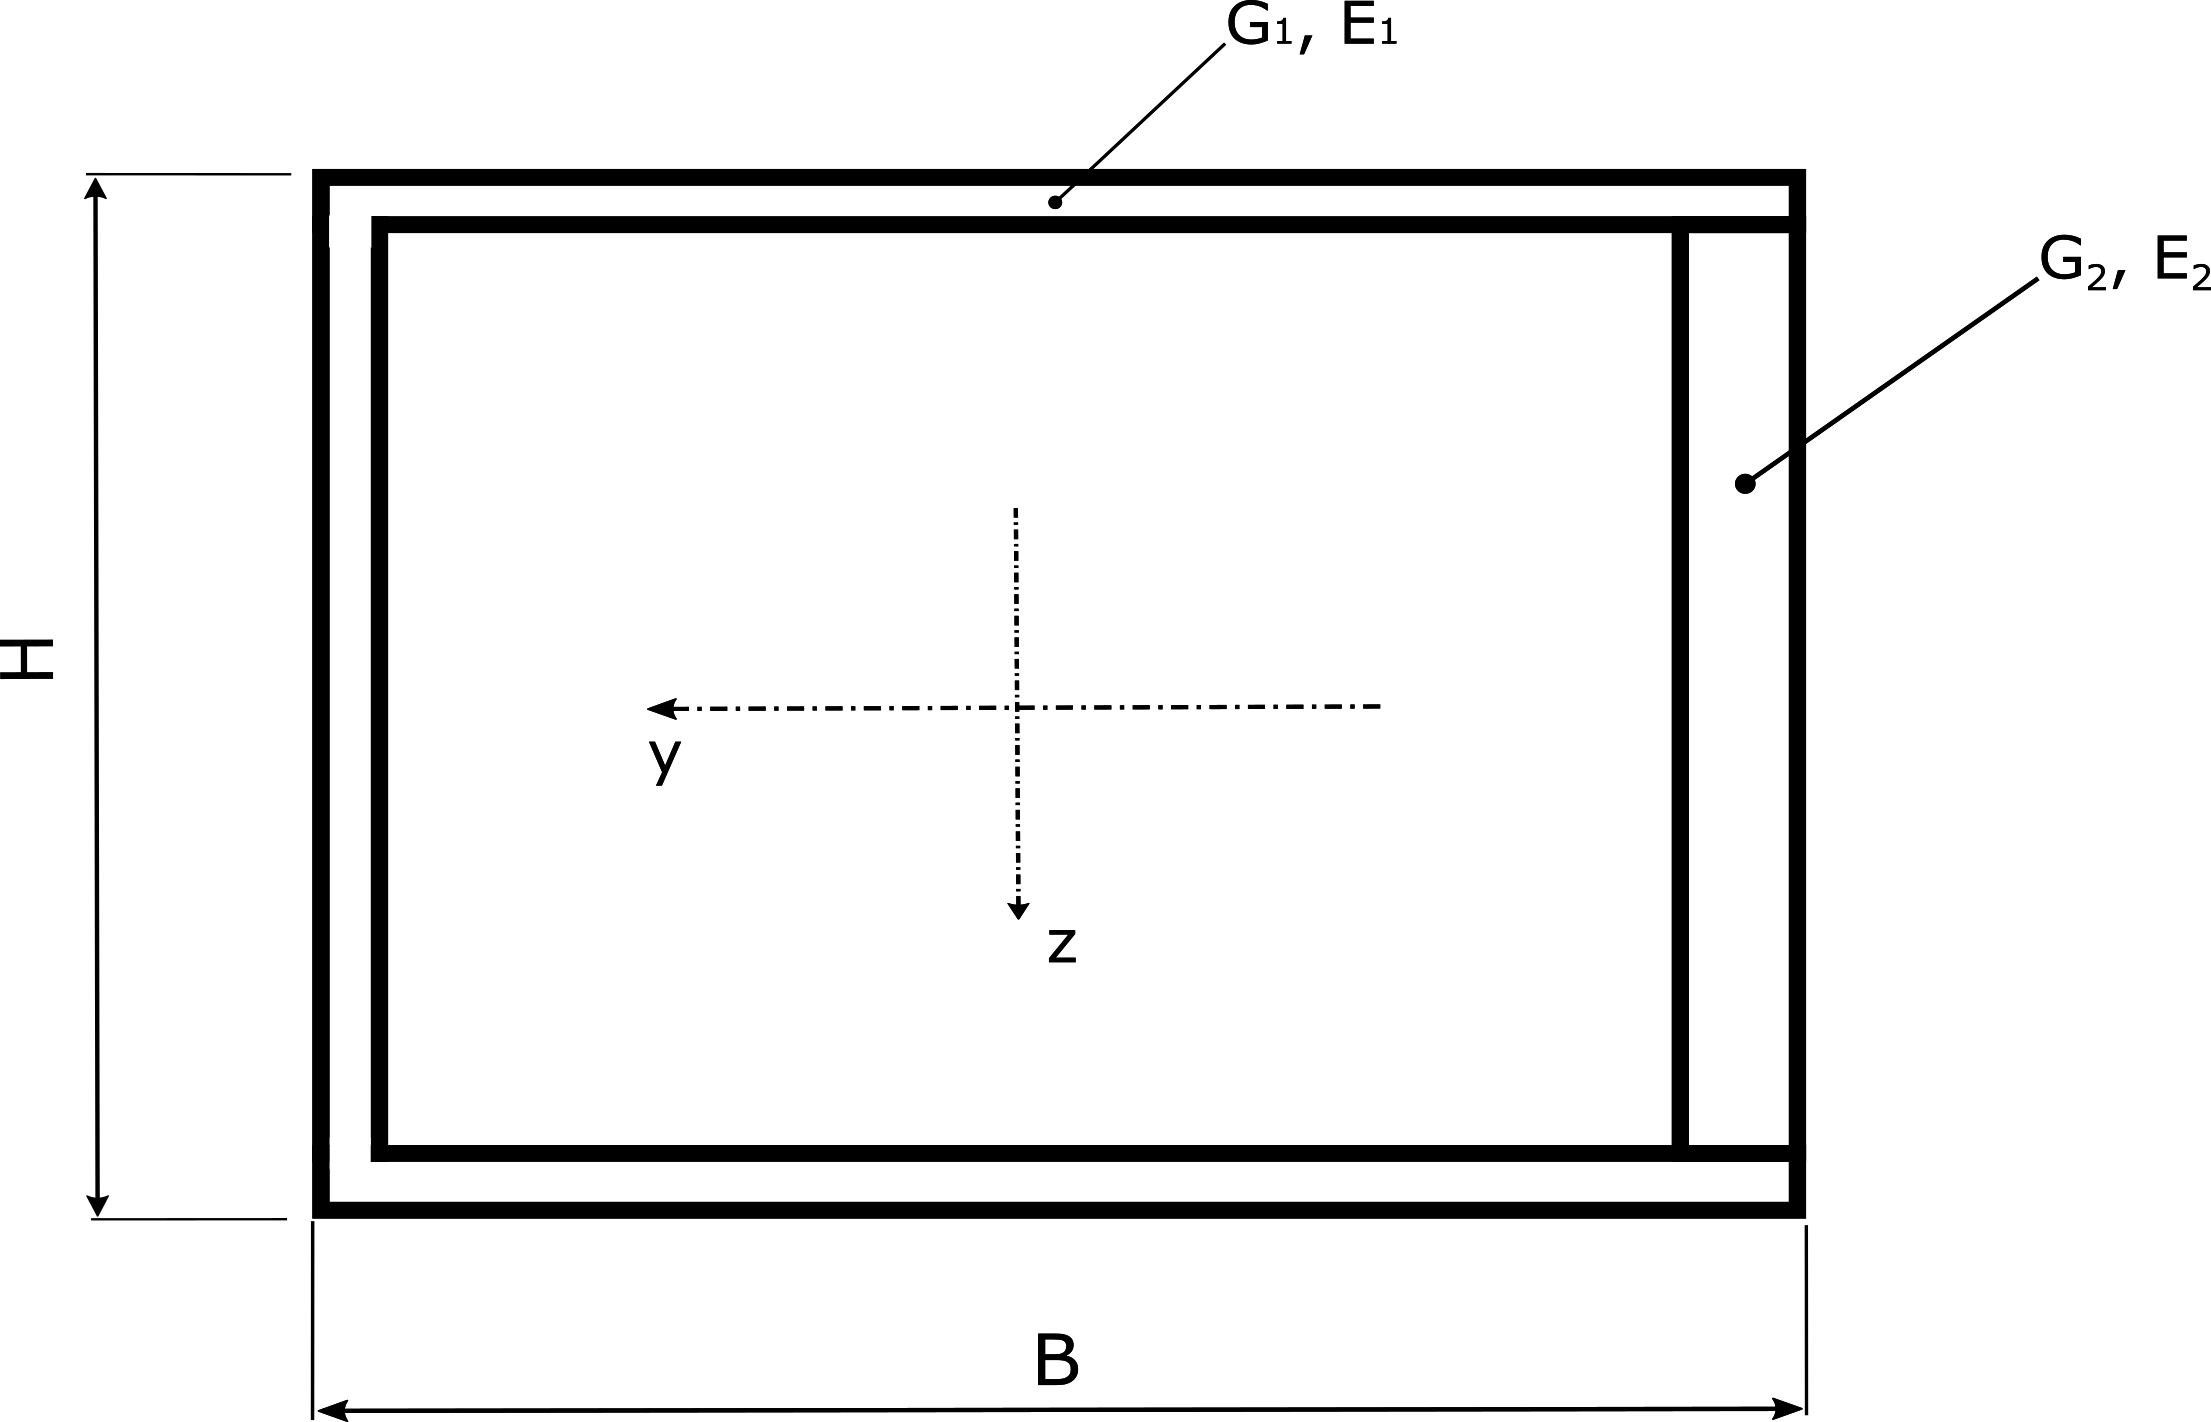
\includegraphics[width=0.8 \textwidth]{model/analyticalBox}
  \caption[Schematic view of the beam closed section]{Schematic view of the beam closed section. The dimensions are given by the width $B$ and the height $H$. For the upper, lower and left elements, the shear modulus and the elastic modulus are given by $G_1$ and $E_1$, respectively. For the right element, the same mechanical properties are given by $G_2$ and $E_2$.}\label{fig:analyticalBox}
\end{figure}

%Torsional stiffness

\begin{equation}\label{eq:torStiff}
  G I_t = \frac{4 A_0^2}{\oint \frac{\mathrm{d} s}{G(s) t(s)}}
\end{equation}

%Equations for the static moment and the flexural stiffness along the $y$ axis $\Phi_y$ (3.17, 3.18, 3.19)
Furthermore, the shear flow distribution in the beam will be calculated. This shear flow $q_\mathrm{C}(s)$ is dependent on the position parameter $s$ and is given by Equation \ref{eq:shearFlowEquation} for the case of beam with closed double symmetric transversal section.
%
\begin{equation}\label{eq:shearFlowEquation}
  q_\mathrm{C}(s) - q_0 = - \frac{Q_z}{\Phi_y} S_{E_y}(s)
\end{equation}
%
where $Q_z$ is the force applied in the z direction and $\Phi_y$ is the flexural stiffness given by Equation \ref{eq:flexuralStiffness}. Additionally, $S_{E_y}$ is the so called static moment or first moment of area, which is calculated through the integral shown in Equation \ref{eq:staticMoment}. In case of open section, the shear flow at the boundary $q_0$ that results from the torsion of the beam, is zero. For the remaining cases, the shear flow at the boundary $q_0$ can be calculated using the Equation \ref{eq:constantShearFlow}.
%
\begin{equation}\label{eq:flexuralStiffness}
  \Phi_y = \int \int E(y,z) z^2 \mathrm{d}y \mathrm{d}z
\end{equation}
%
\begin{equation}\label{eq:staticMoment}
  S_{E_y}(s) = \int_0^s E(s) t(s) z(s) \mathrm{d}s
\end{equation}
%
\begin{equation}\label{eq:constantShearFlow}
  q_0 = \frac{Q_z}{\Phi_y} \frac{ \oint_s \frac{S_{E_y}(s)}{G(s) t(s)} \mathrm{d}s }{ \oint_s \frac{1}{G(s) t(s)} \mathrm{d}s }
\end{equation}

Now, the shear centre position in the beam transversal section will be calculated for the case of open section. Given that beam mechanical properties and geometrical dimensions are symmetric around y axis, the shear centre position in the z axis will be $z_{\mathrm{SC}} = 0$. On the other hand, the shear centre position in the y axis will be given by the Equation \ref{eq:shearCentrePosition}.
%
\begin{equation}\label{eq:shearCentrePosition}
  y_{\mathrm{SC,open}} = \frac{1}{Q_z} \oint_s q_\mathrm{C}(s) r(s) \mathrm{d}s
\end{equation}
%
where $r$ represents the perpendicular distance to the coordinate origin.

Now, it is necessary that equilibrium exists between the torsional moment due to the shift of the shear centre (caused during the opening of the profile) and the moment due to the torsional shear flow of the closed profile. This condition can be mathematically expressed through Equation \ref{eq:shearCentrePositionMoment}. 
%
\begin{eqnarray}\label{eq:shearCentrePositionMoment}
% \nonumber % Remove numbering (before each equation)
  M_\mathrm{t} &=& Q_\mathrm{z} (y_{\mathrm{SC,open}} - y_{\mathrm{SC,closed}}) \nonumber \\
  &=& 2 A_0 q_0
\end{eqnarray}
%
%where it has been considered that a positive moment $M_\mathrm{t}$ along the x direction produces a constant shear flow distribution which has negative sign given the shear flow distribution definition in the present text.

Finally, the total shear flow $q(s)$ results from the superposition of the shear flow of the open profile $q_\mathrm{C}$ and the constant shear flow due to torsion $q_0$, as shown in the Equation \ref{eq:totalShearFlow}.
%
\begin{equation}\label{eq:totalShearFlow}
  q(s) = q_\mathrm{C}(s) - q_0 %before it was: q_\mathrm{C}(s) - q_\mathrm{M}
\end{equation}

\subsection{Parametric study} \label{subsec:parametricStudy} %Reference for this part -> \cite{Raither_basic}

In the present subsection, the variation of the beam properties for different parameter values will be shown. The beam geometry will be characterized through the cross-sectional aspect ratio $B/H$, the thickness ratio $t_2/t_1$ and the slenderness ratio $L/B$. The effect of these parameters on the sectional properties, twist and bending stiffness, and flexural and twisting compliance will be shown. Additionally, the variance of the stiffness ratio $E_1/E_2$ will also be included in the analysis.

\subsubsection{Results} \label{subsubsec:results_parametricStudy}

The influence of the cross-sectional aspect ratio $B/H$ on the torsional stiffness $G I_t$, the shear centre position $y_{\mathrm{SC}}$ and the flexural stiffness $E I_y$ is shown in Figures \ref{fig:GIt-E1overE2-BoverH}, \ref{fig:SC-E1overE2-BoverH} and \ref{fig:EIy-E1overE2-BoverH}, respectively. On its side, the effect of thickness ratio $t_2/t_1$ on the same three beam parameters is shown in Figures \ref{fig:GIt-E1overE2-t2overt1}, \ref{fig:SC-E1overE2-t2overt1} and \ref{fig:EIy-E1overE2-t2overt1}.

Additionally, the effect of the cross-sectional aspect ratio $B/H$ on the deflection and torsional compliance is shown on Figures \ref{fig:woverQ-E1overE2-BoverH} and \ref{fig:phioverQ-E1overE2-BoverH}, respectively. The corresponding plots when analysing the effect of the thickness ratio $t_2/t_1$ on the deflection and torsional compliance are shown on Figures \ref{fig:woverQ-E1overE2-t2overt1} and \ref{fig:phioverQ-E1overE2-t2overt1}, respectively. The beam's torsional compliance will be expressed as fraction of the twist at the tip divided by the vertical force applied, that is $|\phi_{\mathrm{tip}}| / Q$, while the beam deflection compliance will be expressed as fraction of the maximum vertical displacement at the tip divided by the vertical force applied, that is $w_{\mathrm{0,tip}} / Q$.

The effect of the slenderness ratio $L/B$ on the deflection and torsional compliances is shown in Figures \ref{fig:woverQ-E1overE2-LoverB} and \ref{fig:phioverQ-E1overE2-LoverB}, respectively.

%Figures variation of B/H
\begin{figure}[!htpb] %G I_t versus B/H
  \centering
  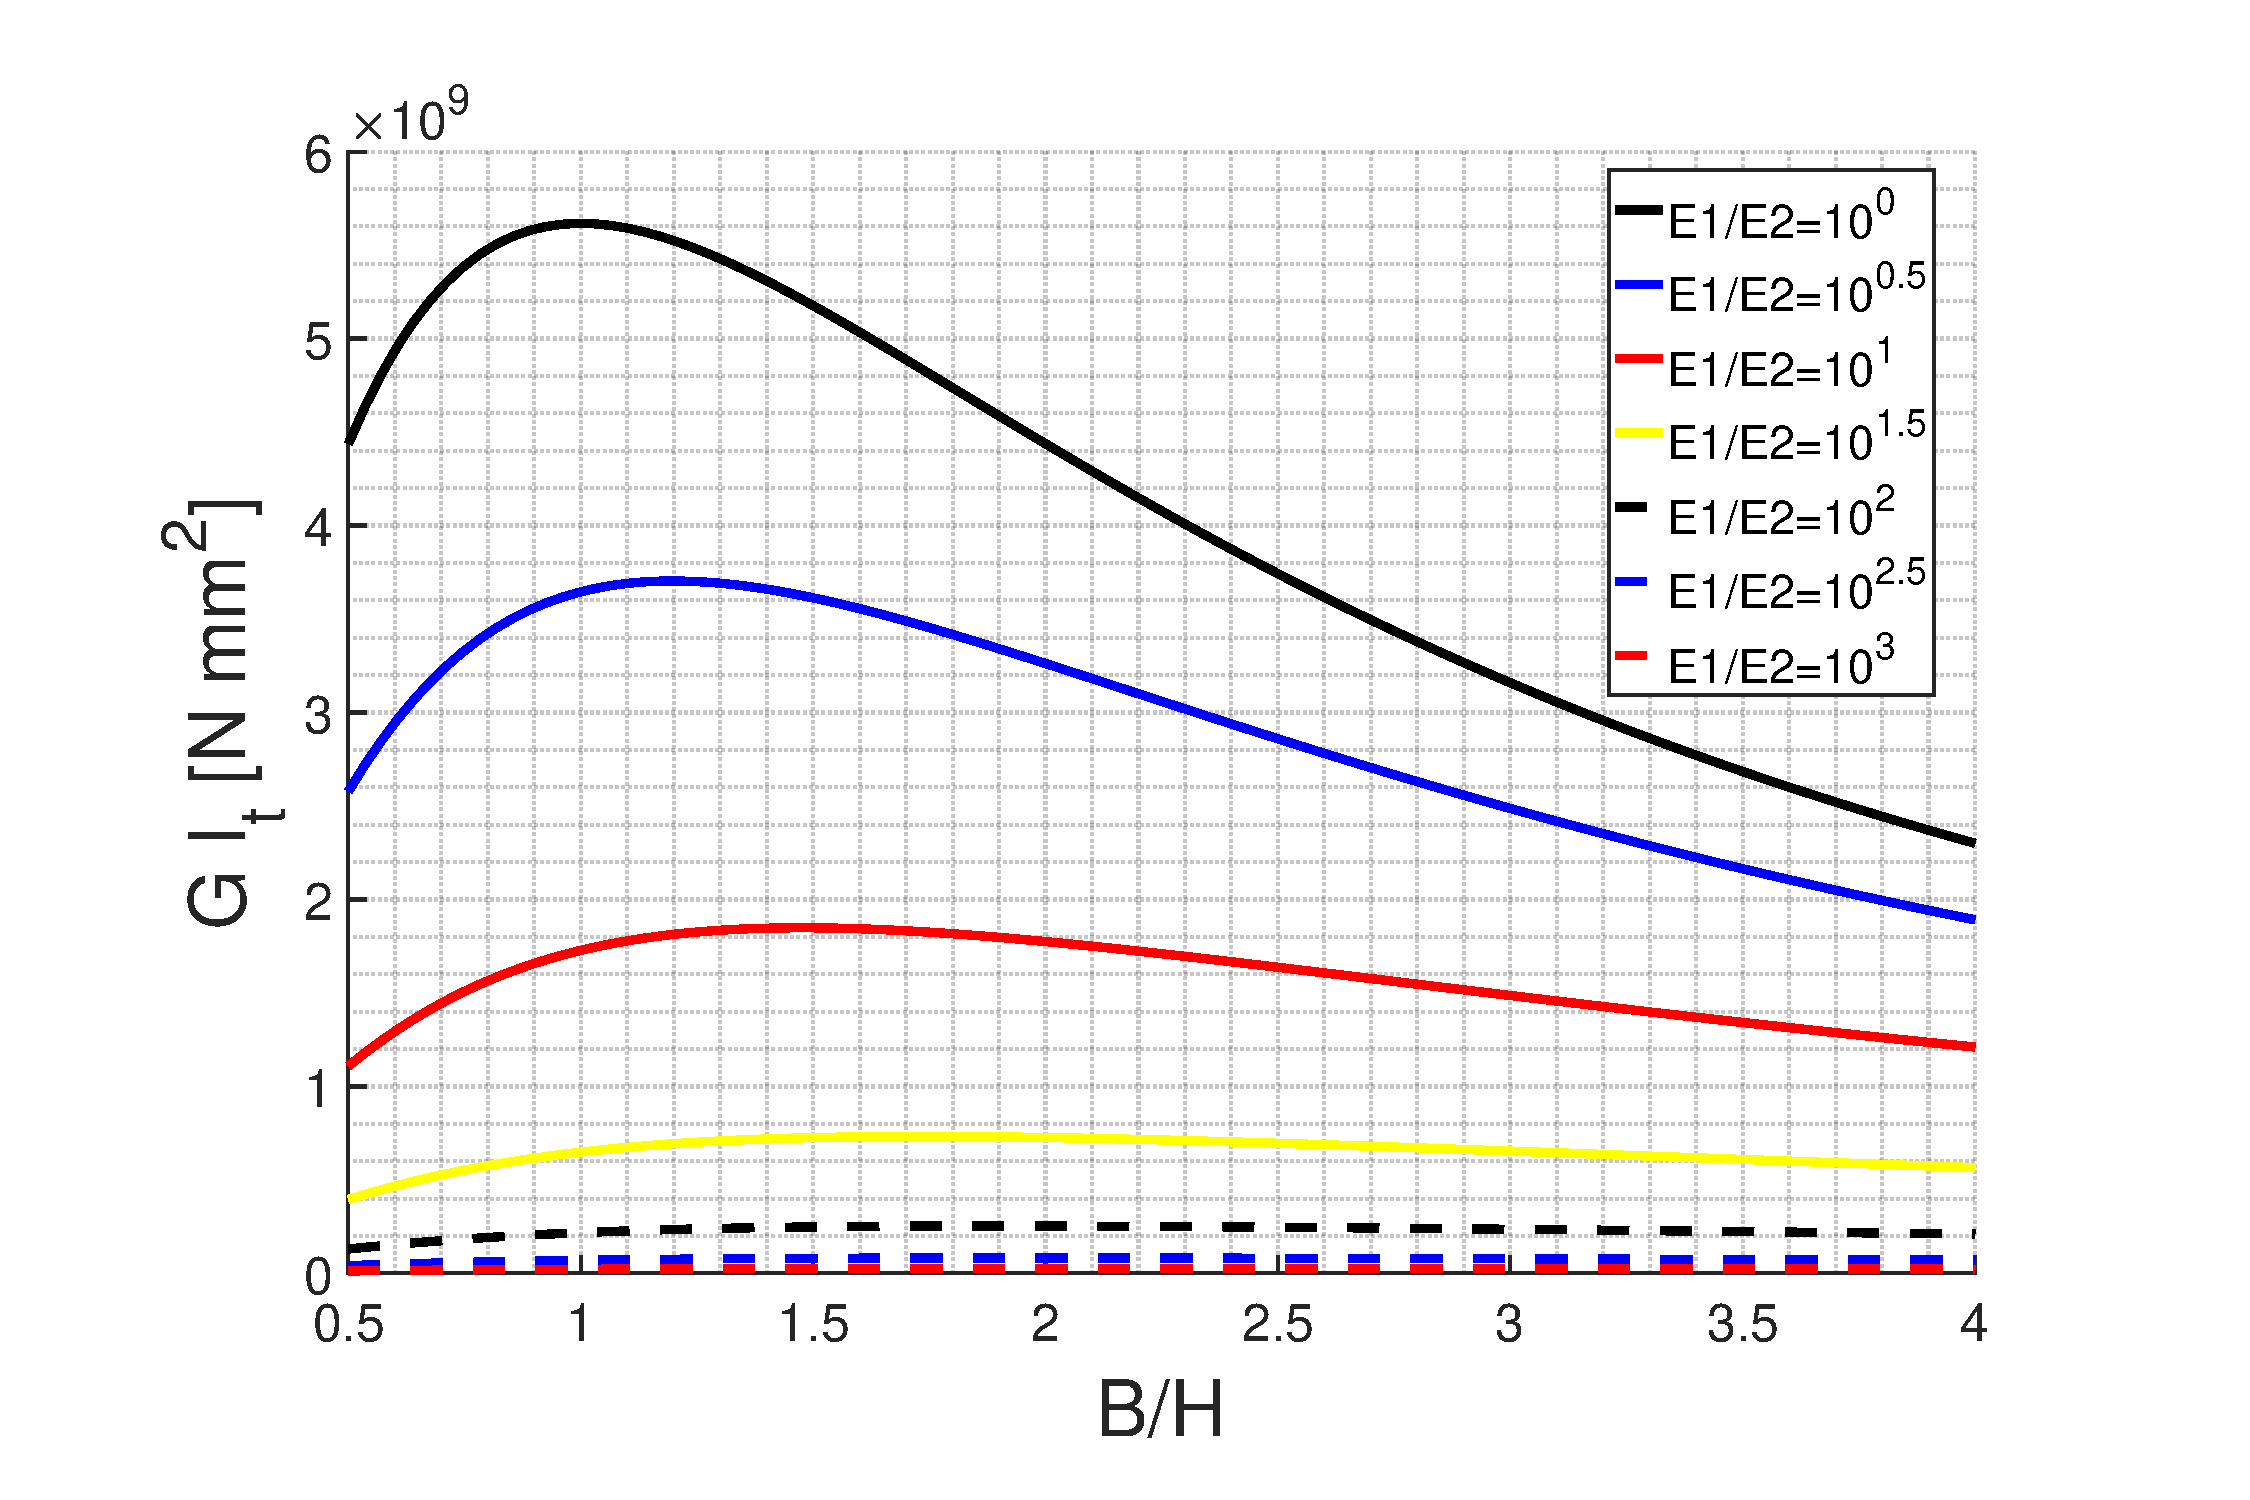
\includegraphics[width=0.8 \textwidth]{../../analytical/figures/GIt-E1overE2-BoverH}
  \caption[Influence of the cross-sectional aspect ratio $B/H$ on the torsional stiffness $GI_t$]{Influence of the cross-sectional aspect ratio $B/H$ on the torsional stiffness $GI_t$ is shown for various values of the stiffness ratio $E_1/E_2$ ranging from $10^0$ to $10^3$. }\label{fig:GIt-E1overE2-BoverH}
\end{figure}

\begin{figure}[!htpb] %Shear centre versus B/H
  \centering
  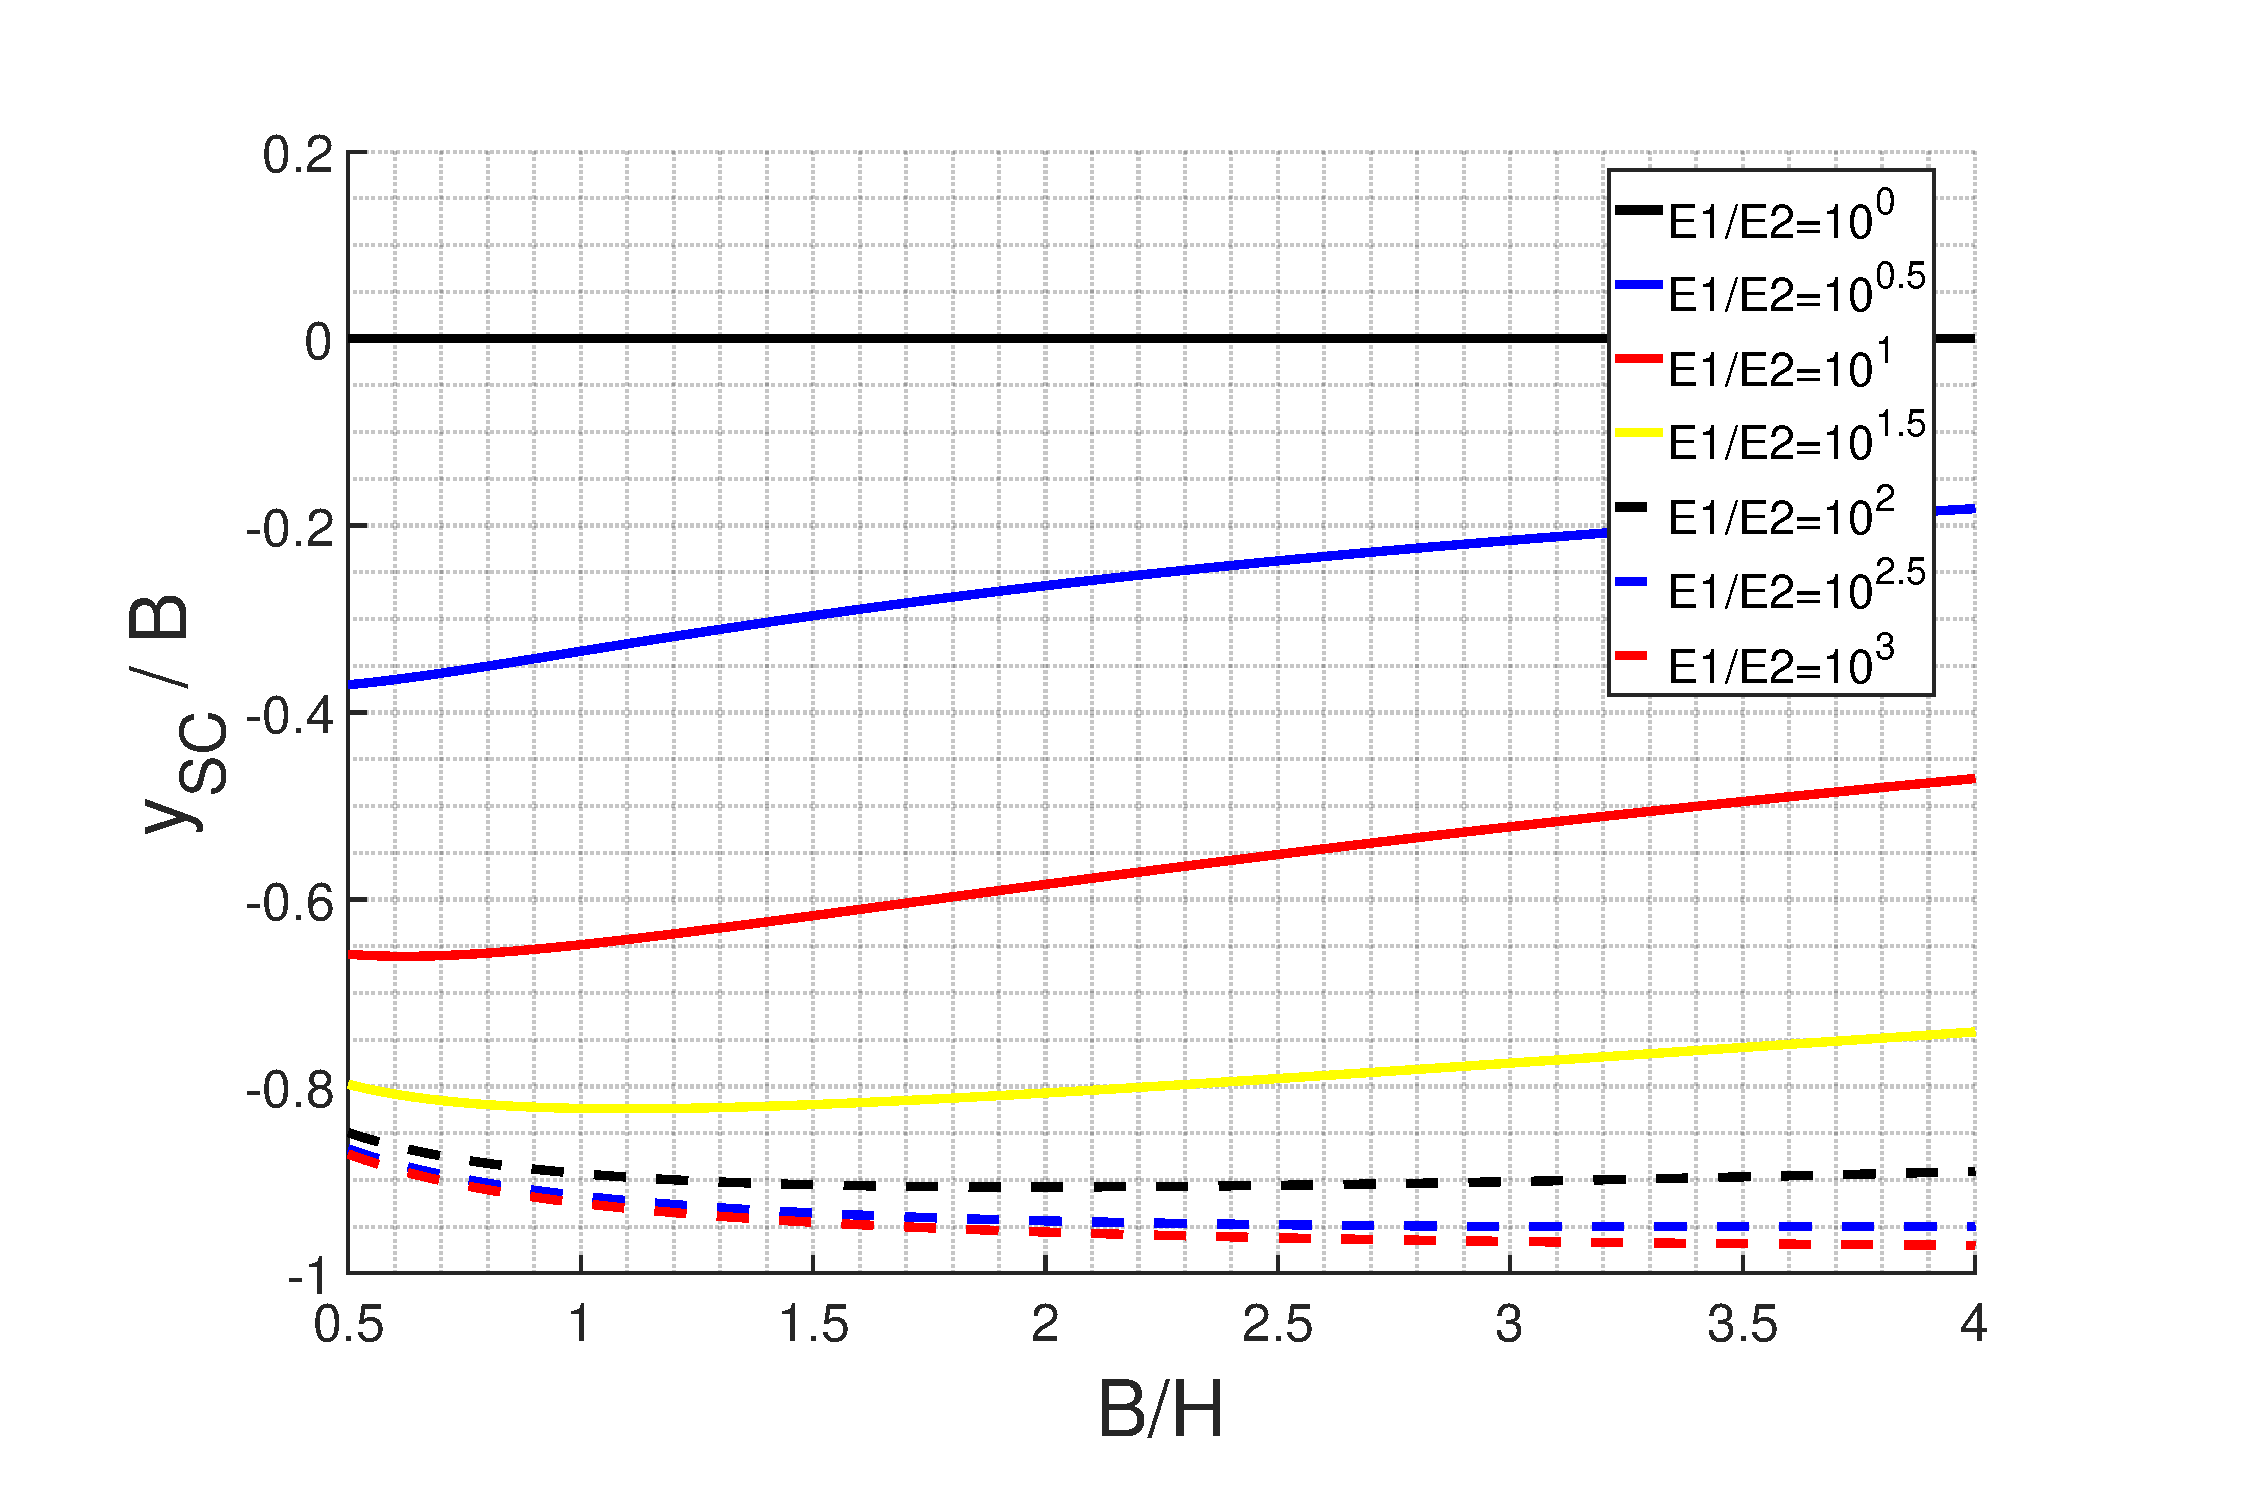
\includegraphics[width=0.8 \textwidth]{../../analytical/figures/SC-E1overE2-BoverH}
  \caption[Influence of the cross-sectional aspect ratio $B/H$ on the dimensionless shear centre position $y_{\mathrm{SC}}/B$]{Influence of the cross-sectional aspect ratio $B/H$ on the dimensionless shear centre position $y_{\mathrm{SC}}/B$ is shown for various values of the stiffness ratio $E_1/E_2$ ranging from $10^0$ to $10^3$. }\label{fig:SC-E1overE2-BoverH}
\end{figure}

\begin{figure}[!htpb] %E I_y = \Phi_y versus B/H
  \centering
  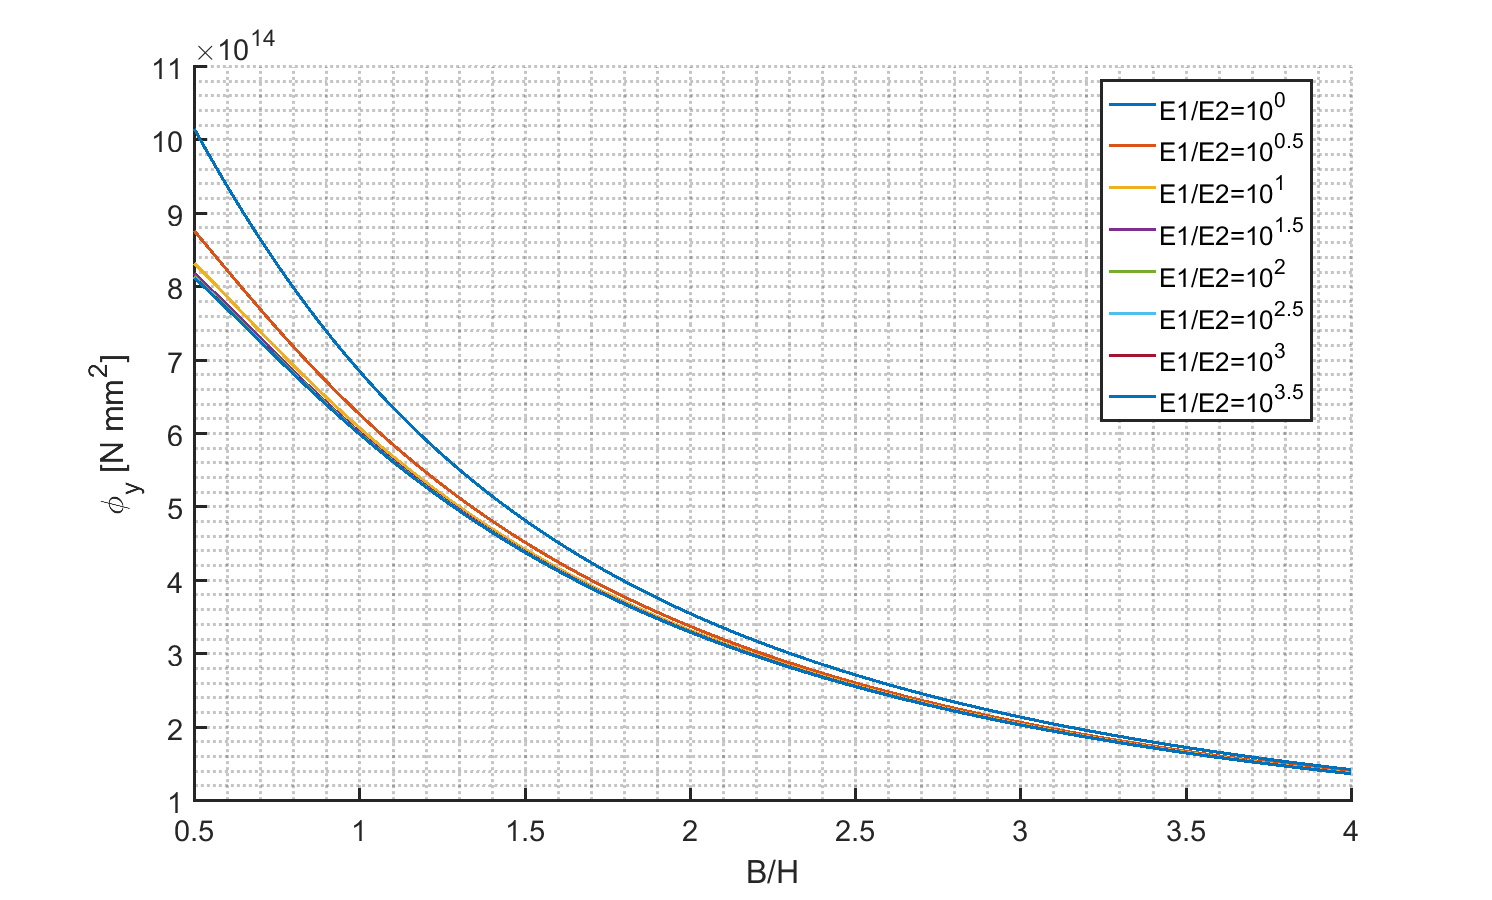
\includegraphics[width=0.8 \textwidth]{../../analytical/figures/EIy-E1overE2-BoverH}
  \caption[Influence of the cross-sectional aspect ratio $B/H$ on the flexural stiffness $EI_y$]{Influence of the cross-sectional aspect ratio $B/H$ on the flexural stiffness $EI_y = \Phi_y$ is shown for various values of the stiffness ratio $E_1/E_2$ ranging from $10^0$ to $10^3$. }\label{fig:EIy-E1overE2-BoverH}
\end{figure}

\begin{figure}[!htpb] %w_0,tip / Q versus B/H, deflection compliance
  \centering
  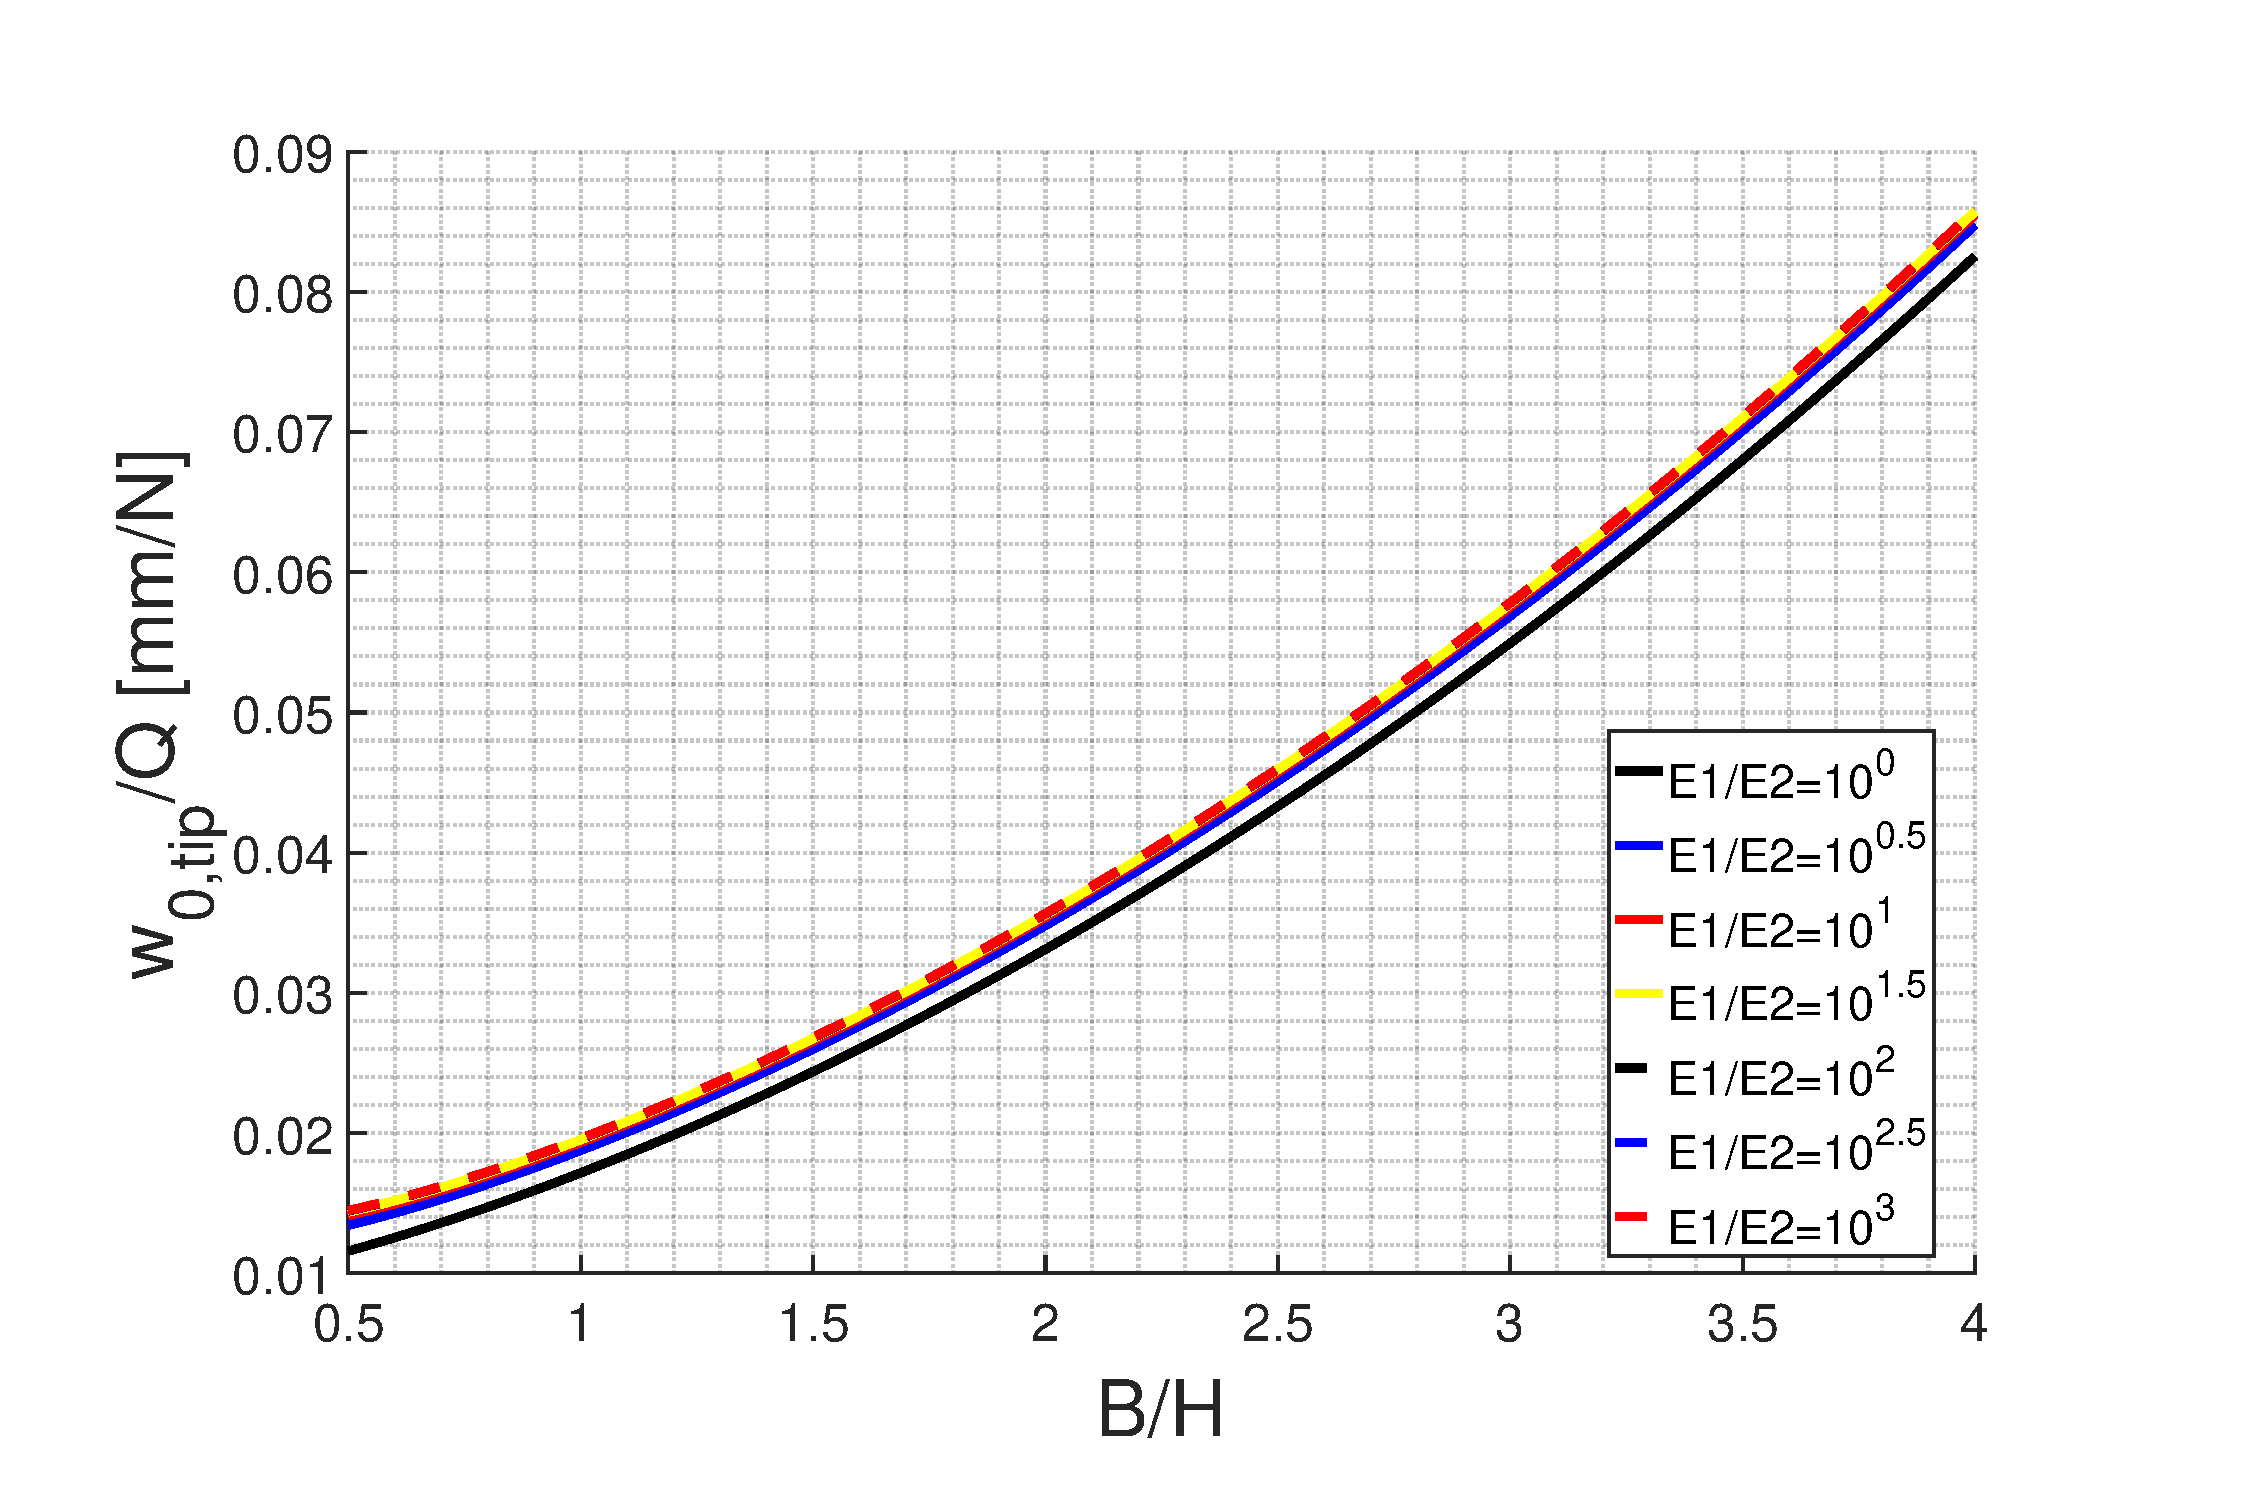
\includegraphics[width=0.8 \textwidth]{../../analytical/figures/woverQ-E1overE2-BoverH}
  \caption[Influence of the cross-sectional aspect ratio $B/H$ on the deflection compliance]{Influence of the cross-sectional aspect ratio $B/H$ on the deflection compliance $w_{\mathrm{0,tip}} / Q$ is shown for various values of the stiffness ratio $E_1/E_2$ ranging from $10^0$ to $10^3$. }\label{fig:woverQ-E1overE2-BoverH}
\end{figure}

\begin{figure}[!htpb] %\phi_tip / Q versus B/H, torsional compliance
  \centering
  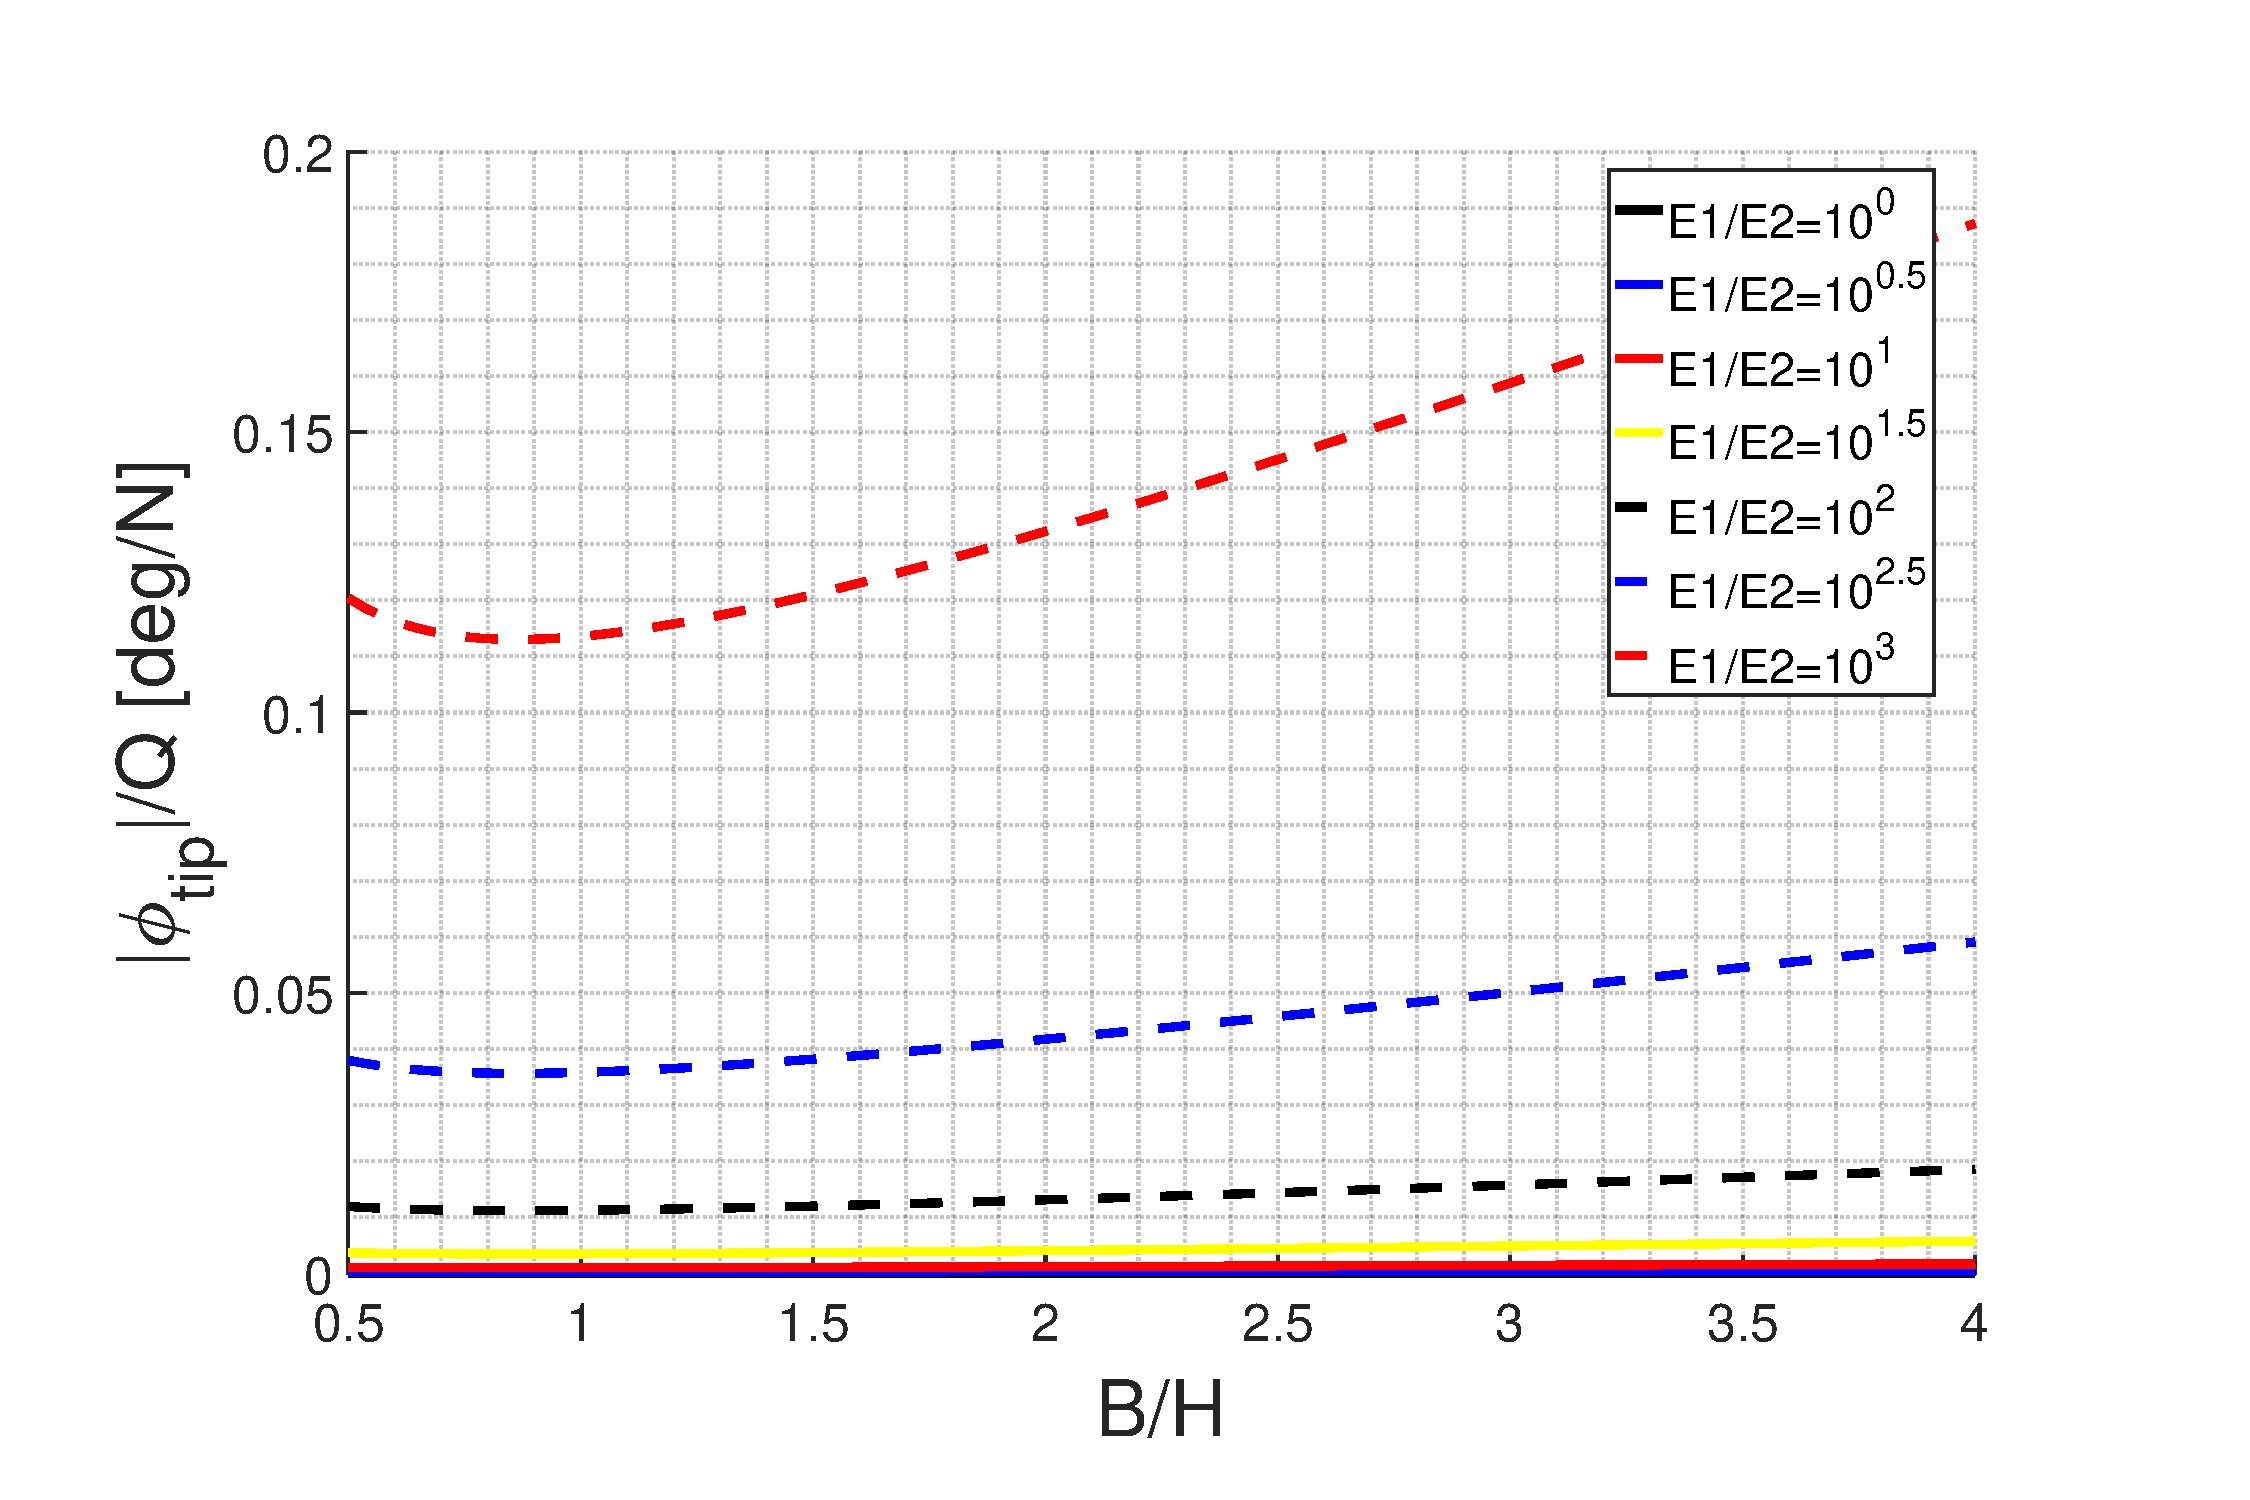
\includegraphics[width=0.8 \textwidth]{../../analytical/figures/phioverQ-E1overE2-BoverH}
  \caption[Influence of the cross-sectional aspect ratio $B/H$ on the torsional compliance]{Influence of the cross-sectional aspect ratio $B/H$ on the torsional compliance $|\phi_{\mathrm{tip}}| / Q$ is shown for various values of the stiffness ratio $E_1/E_2$ ranging from $10^0$ to $10^3$. }\label{fig:phioverQ-E1overE2-BoverH}
\end{figure}

%%%% Figures variation of t2/t1
\begin{figure}[!htpb] %G I_t versus t2/t1
  \centering
  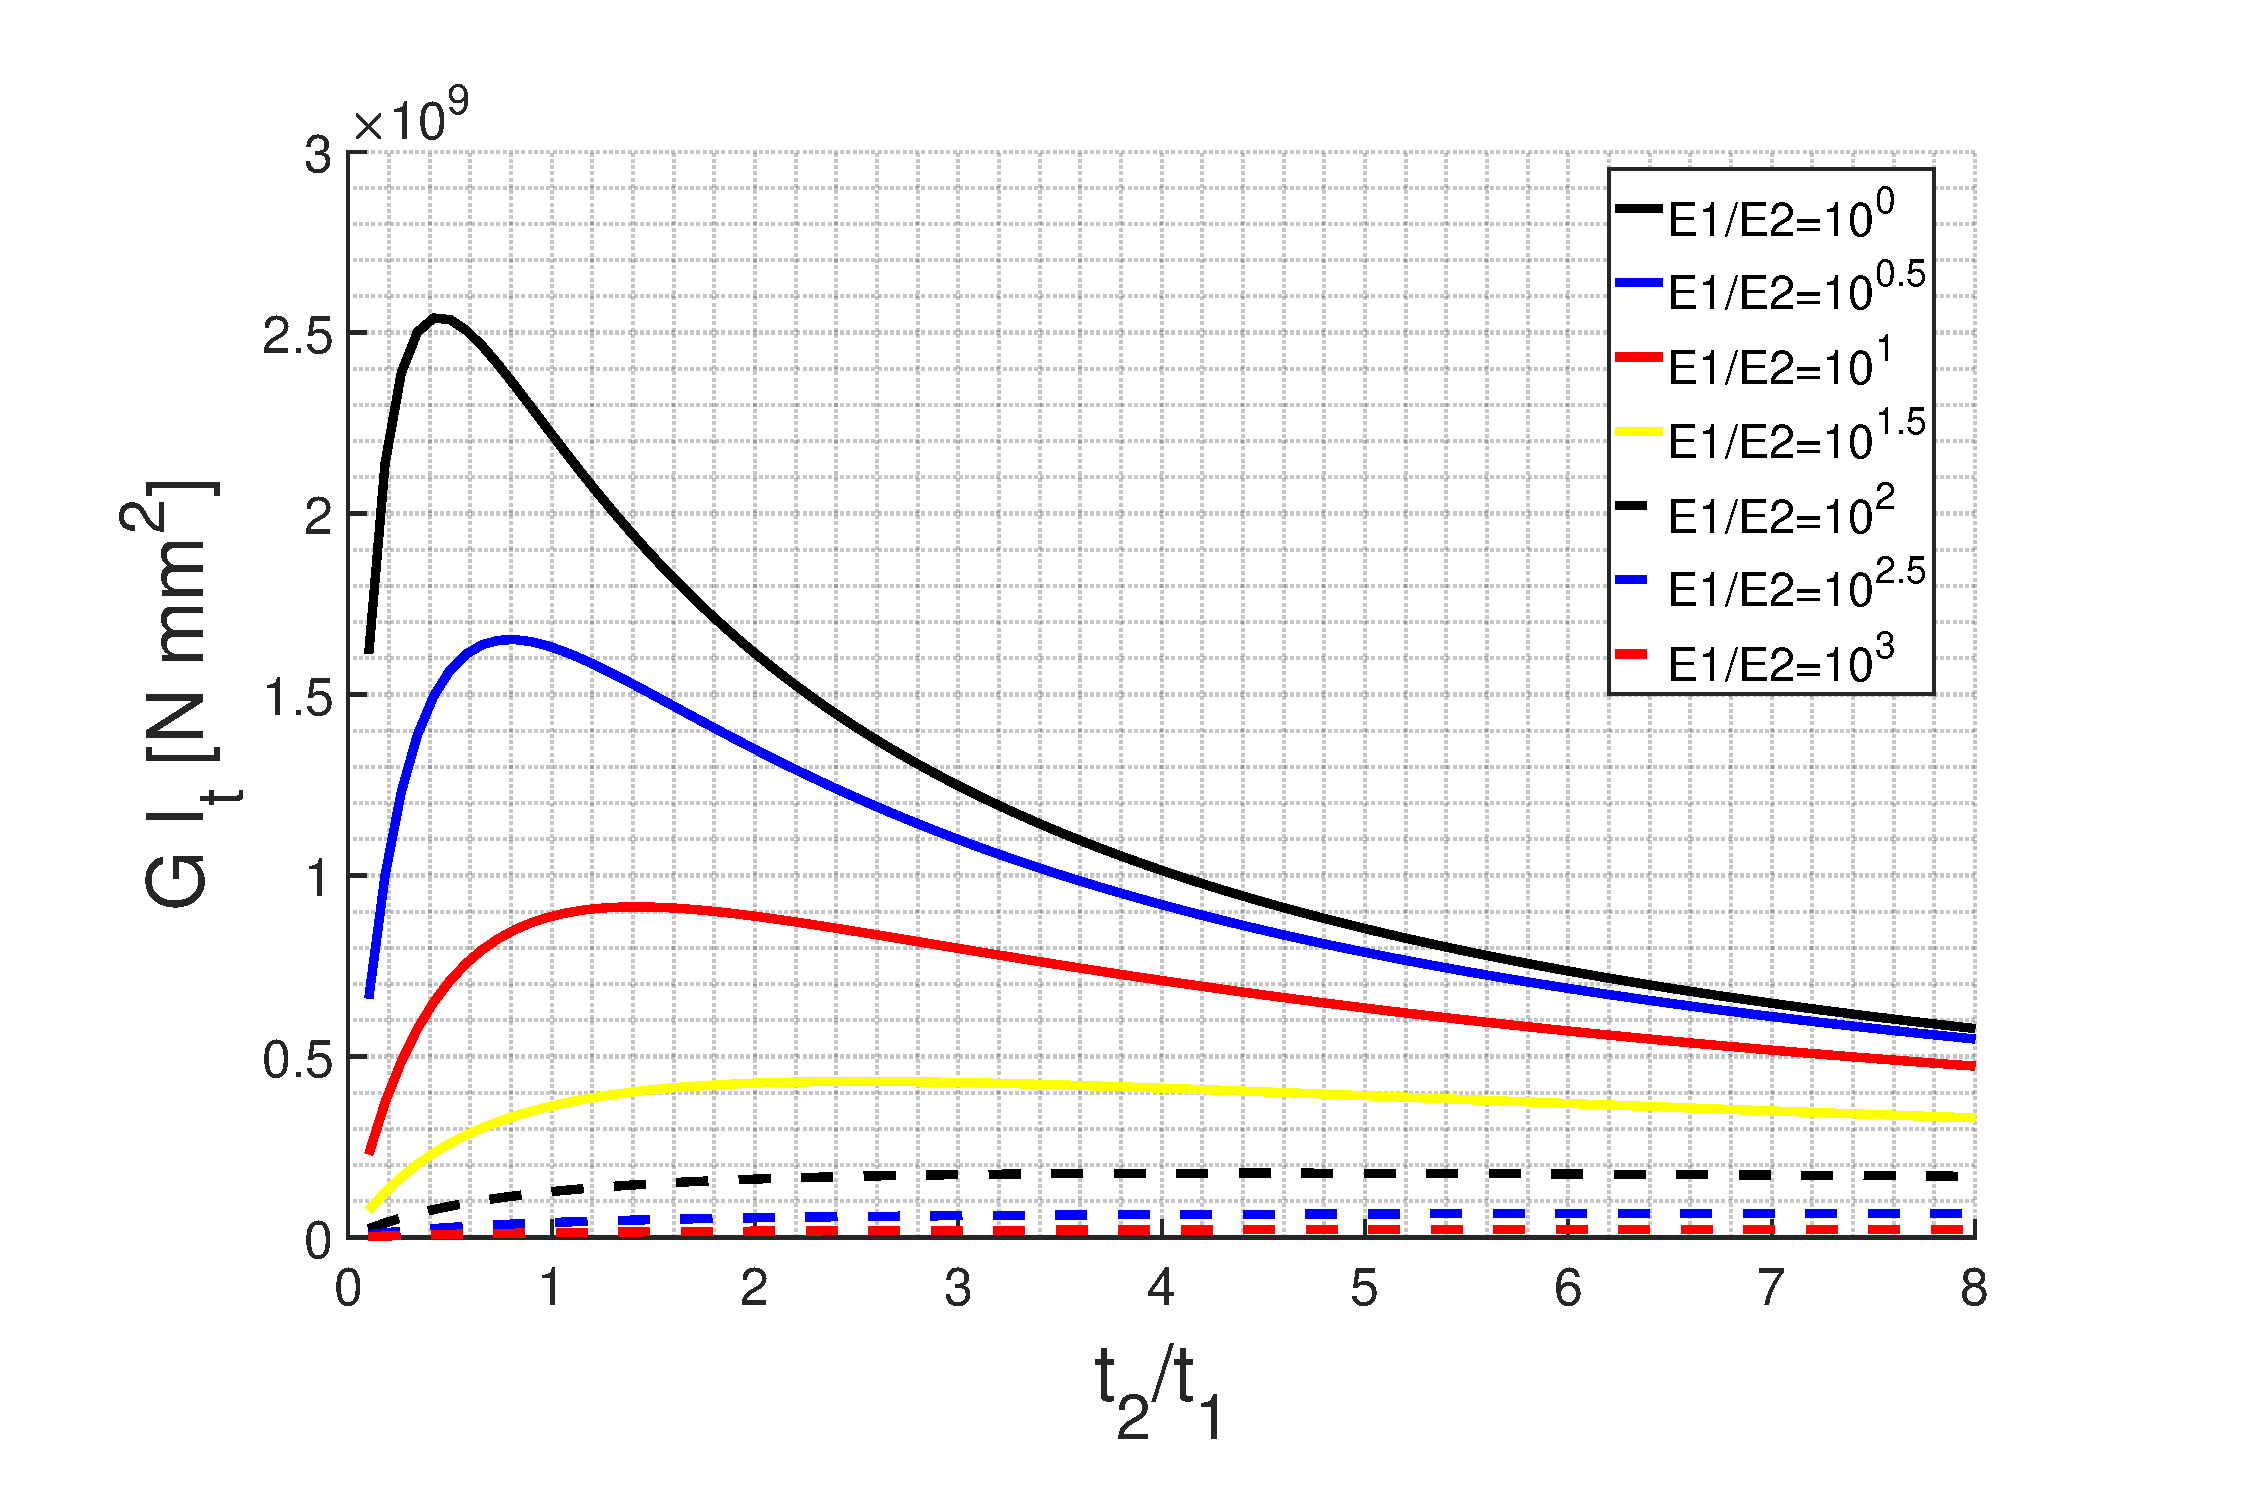
\includegraphics[width=0.8 \textwidth]{../../analytical/figures/GIt-E1overE2-t2overt1}
  \caption[Influence of the wall thickness ratio $t_2/t_1$ on the torsional stiffness $GI_t$]{Influence of the wall thickness ratio $t_2/t_1$ on the torsional stiffness $GI_t$ shown for various values of the stiffness ratio $E_1/E_2$ ranging from $10^0$ to $10^3$. }\label{fig:GIt-E1overE2-t2overt1}
\end{figure}

\begin{figure}[!htpb] %Shear centre versus t2/t1
  \centering
  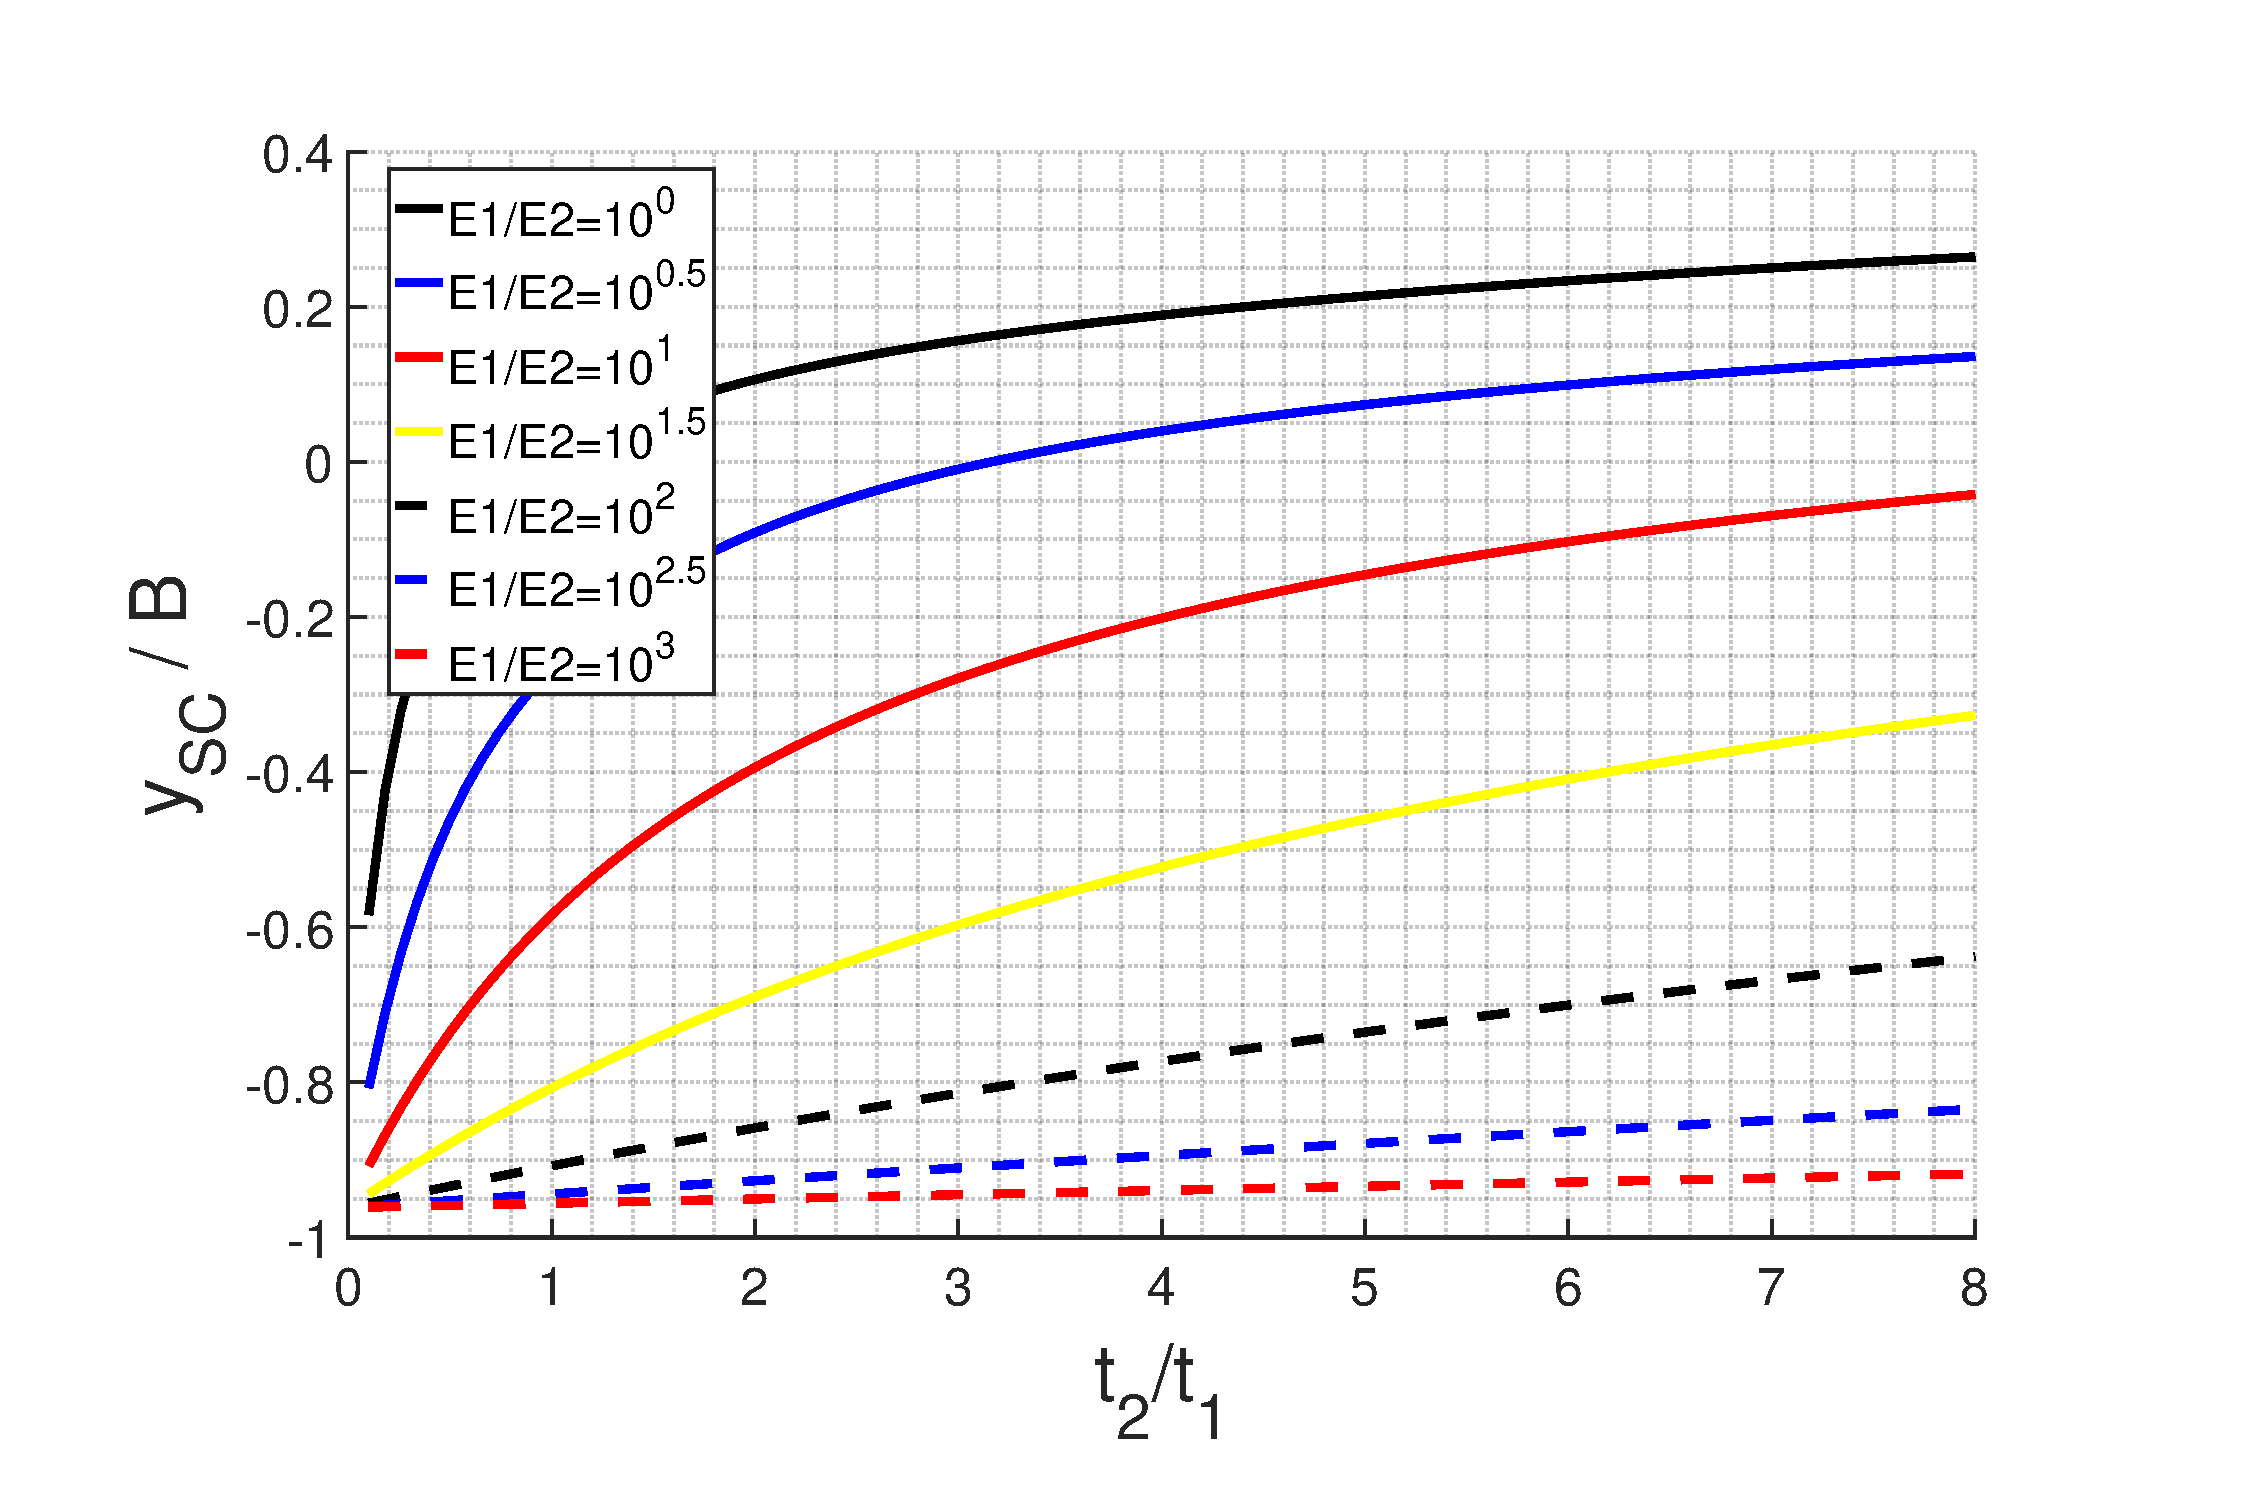
\includegraphics[width=0.8 \textwidth]{../../analytical/figures/SC-E1overE2-t2overt1}
  \caption[Influence of the wall thickness ratio $t_2/t_1$ on the dimensionless shear centre position $y_{\mathrm{SC}}/B$]{Influence of the wall thickness ratio $t_2/t_1$ on the dimensionless shear centre position $y_{\mathrm{SC}}/B$ shown for various values of the stiffness ratio $E_1/E_2$ ranging from $10^0$ to $10^3$. }\label{fig:SC-E1overE2-t2overt1}
\end{figure}

\begin{figure}[!htpb] %E I_y = \Phi_y versus t2/t1
  \centering
  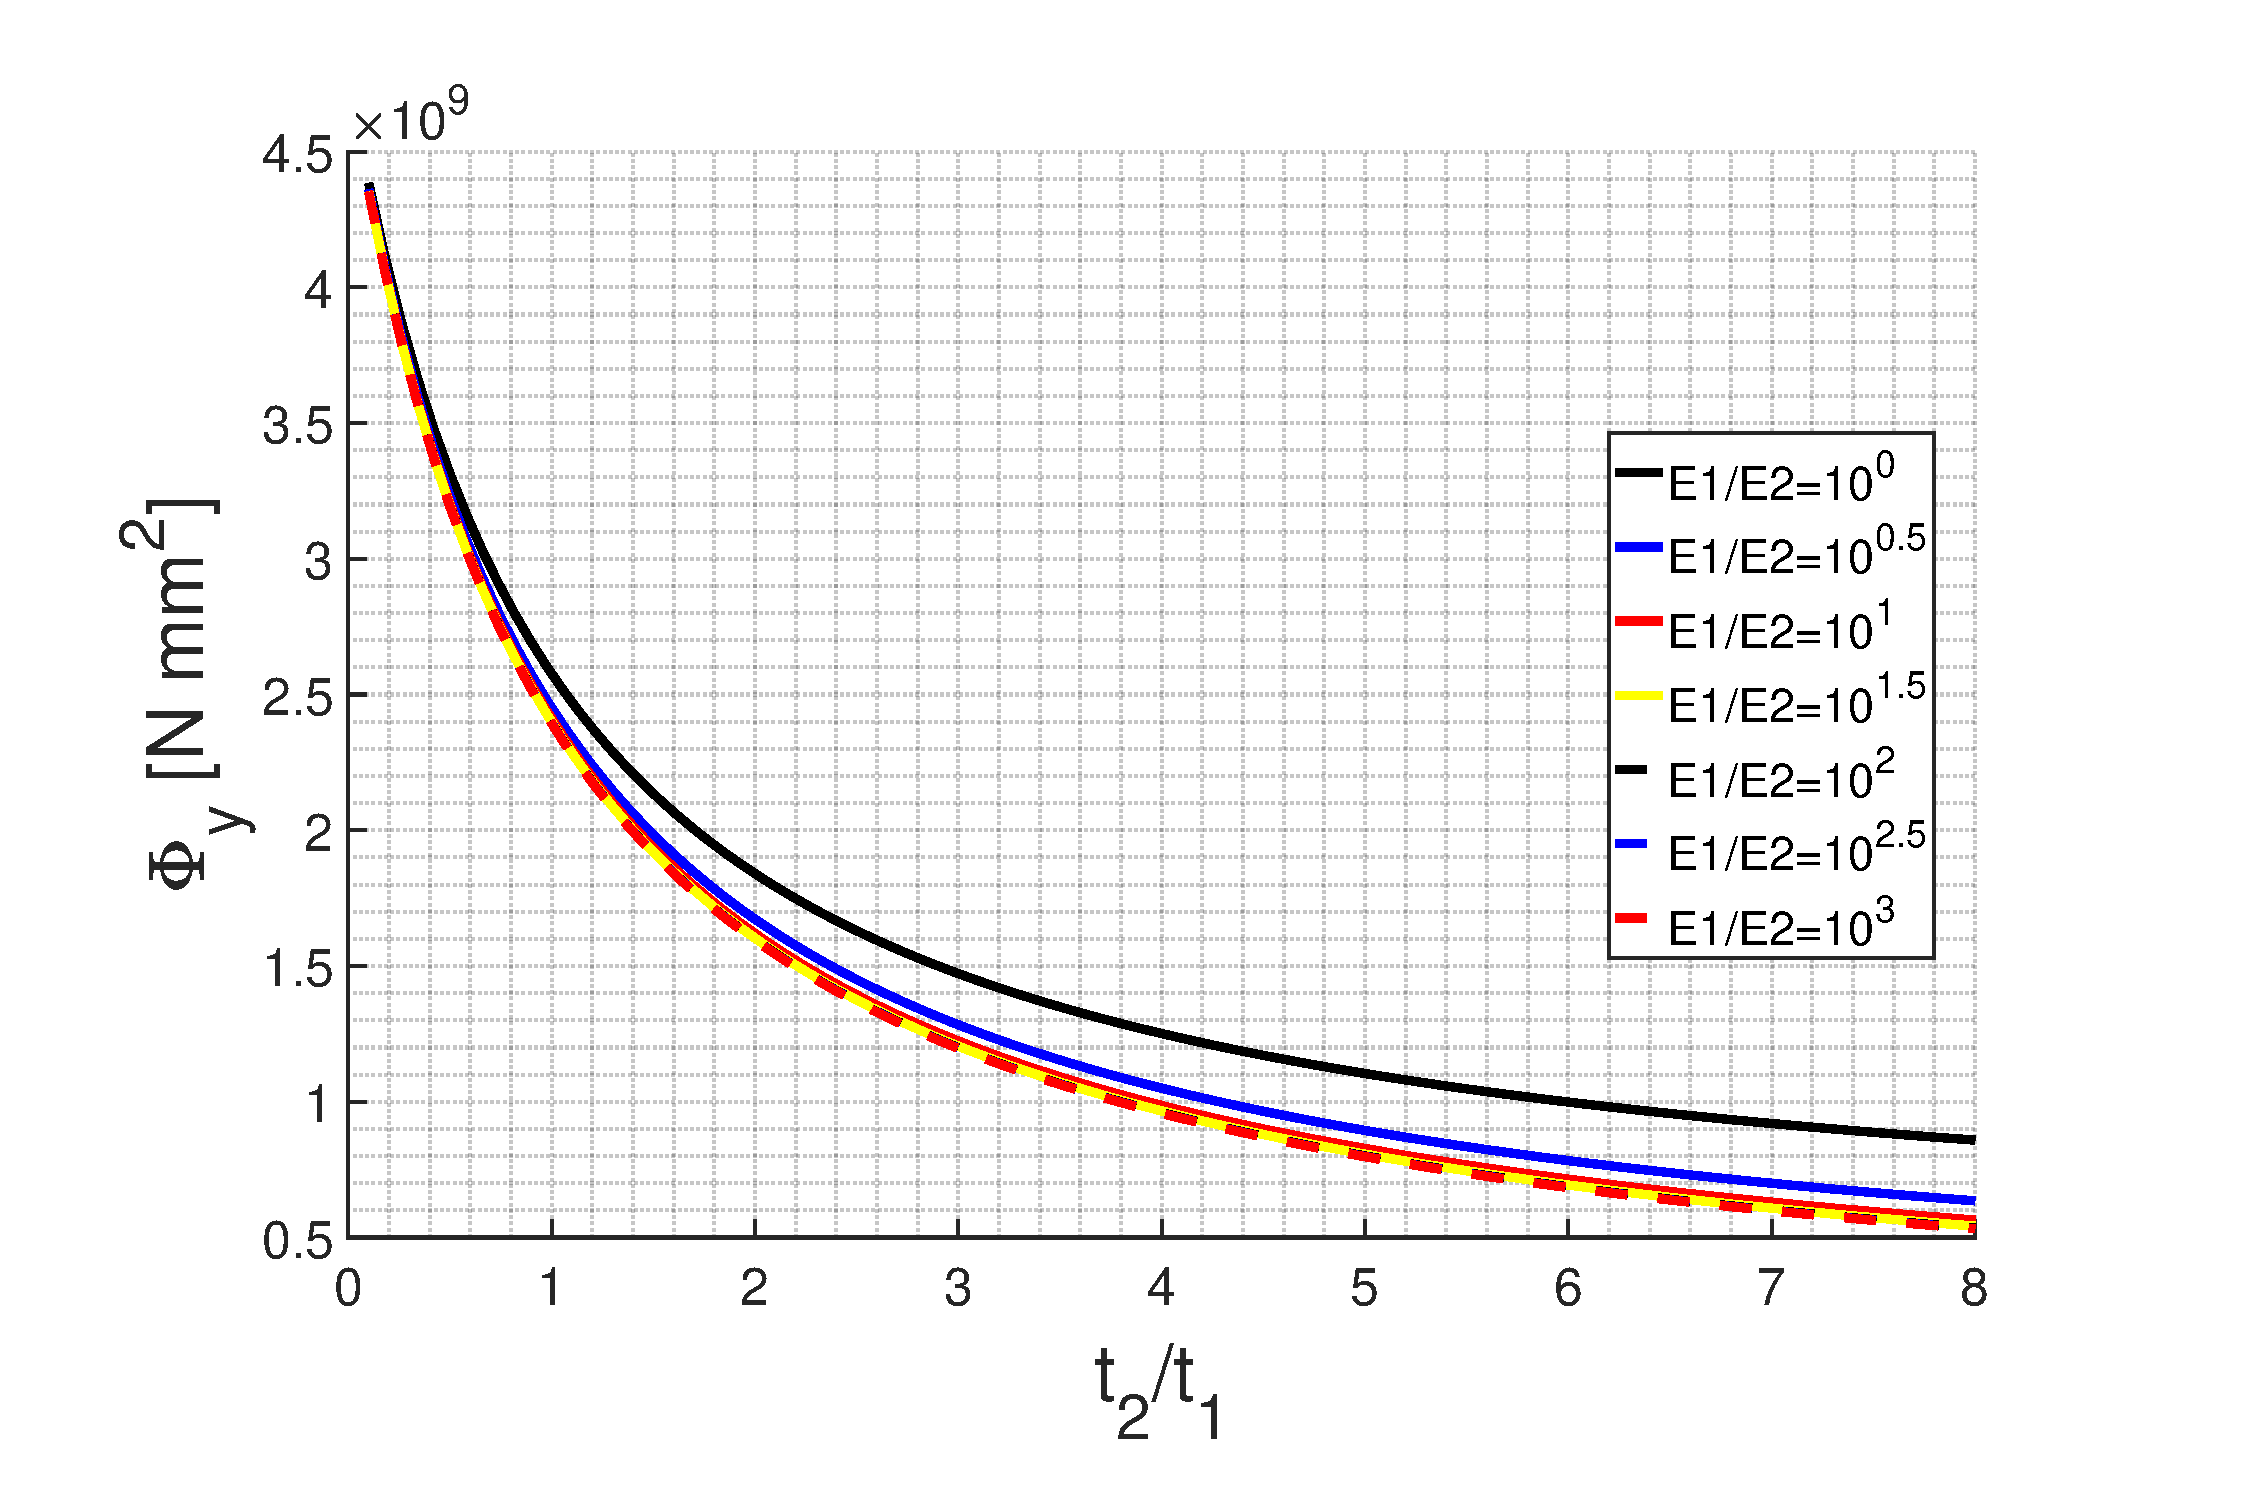
\includegraphics[width=0.8 \textwidth]{../../analytical/figures/EIy-E1overE2-t2overt1}
  \caption[Influence of the wall thickness ratio $t_2/t_1$ on the flexural stiffness $EI_y$]{Influence of the wall thickness ratio $t_2/t_1$ on the flexural stiffness $EI_y = \Phi_y$ shown for various values of the stiffness ratio $E_1/E_2$ ranging from $10^0$ to $10^3$. }\label{fig:EIy-E1overE2-t2overt1}
\end{figure}

\begin{figure}[!htpb] %w_0,tip / Q versus t2/t1, deflection compliance
  \centering
  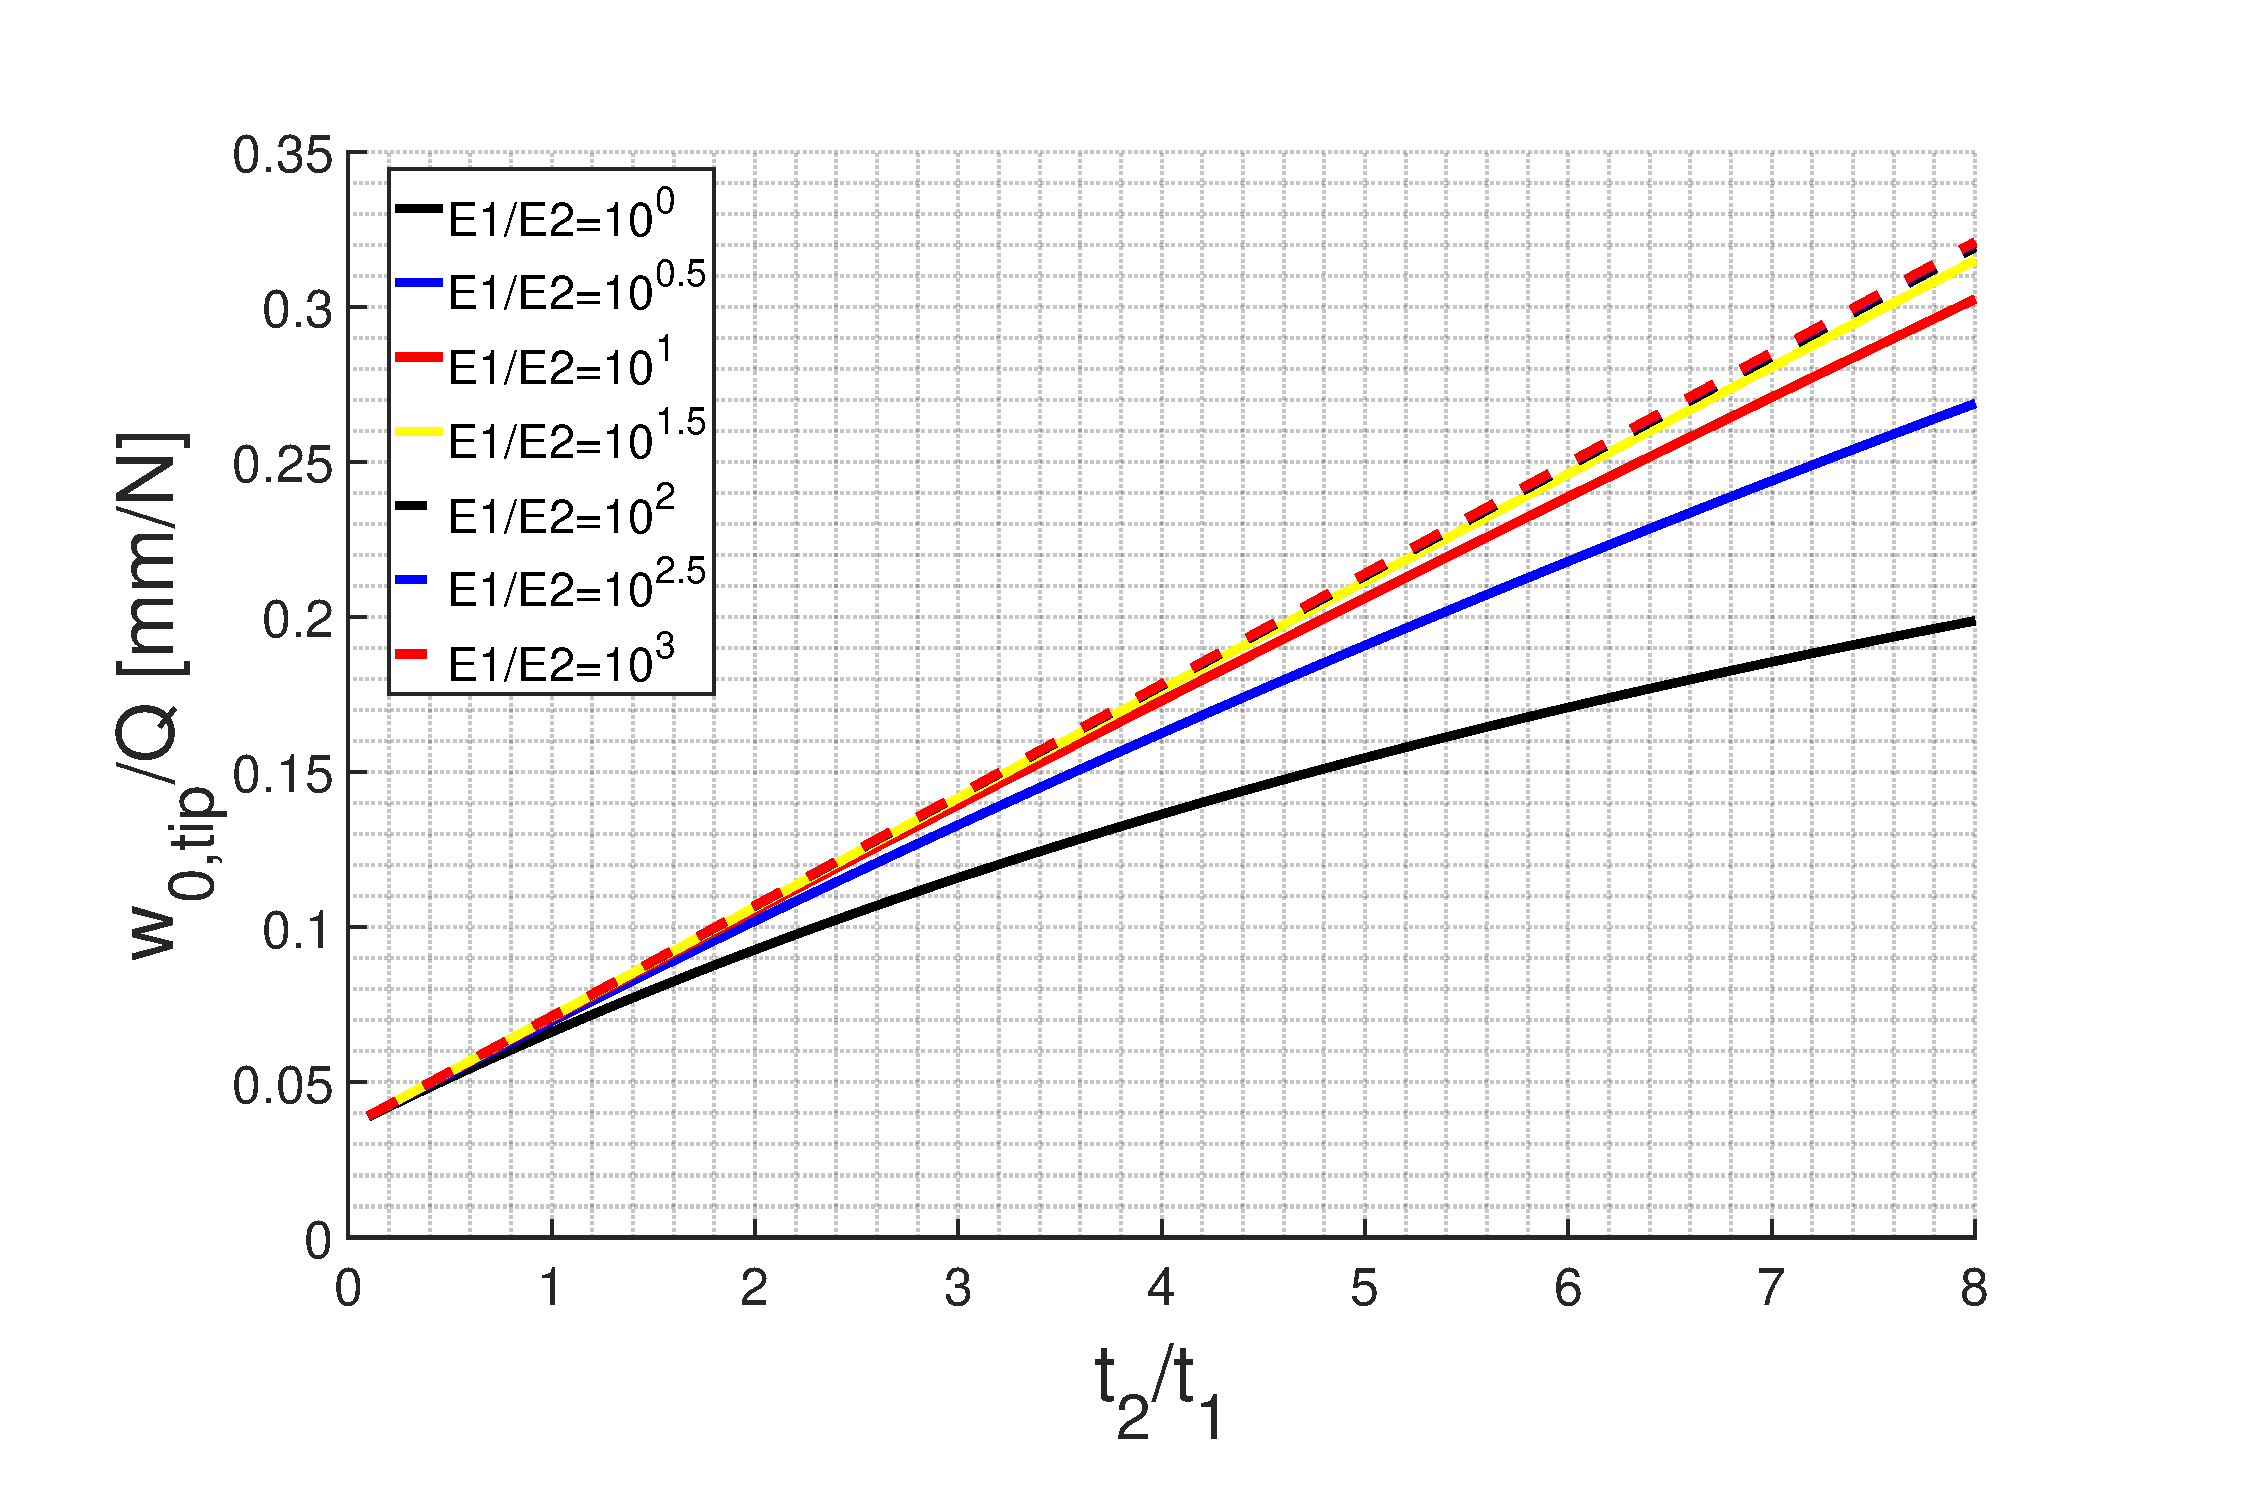
\includegraphics[width=0.8 \textwidth]{../../analytical/figures/woverQ-E1overE2-t2overt1}
  \caption[Influence of the thickness ratio $t2/t1$ on the deflection compliance]{Influence of the thickness ratio $t2/t1$ on the deflection compliance $w_{\mathrm{0,tip}} / Q$ is shown for various values of the stiffness ratio $E_1/E_2$ ranging from $10^0$ to $10^3$. }\label{fig:woverQ-E1overE2-t2overt1}
\end{figure}

\begin{figure}[!htpb] %\phi_tip / Q versus t2/t1, torsional compliance
  \centering
  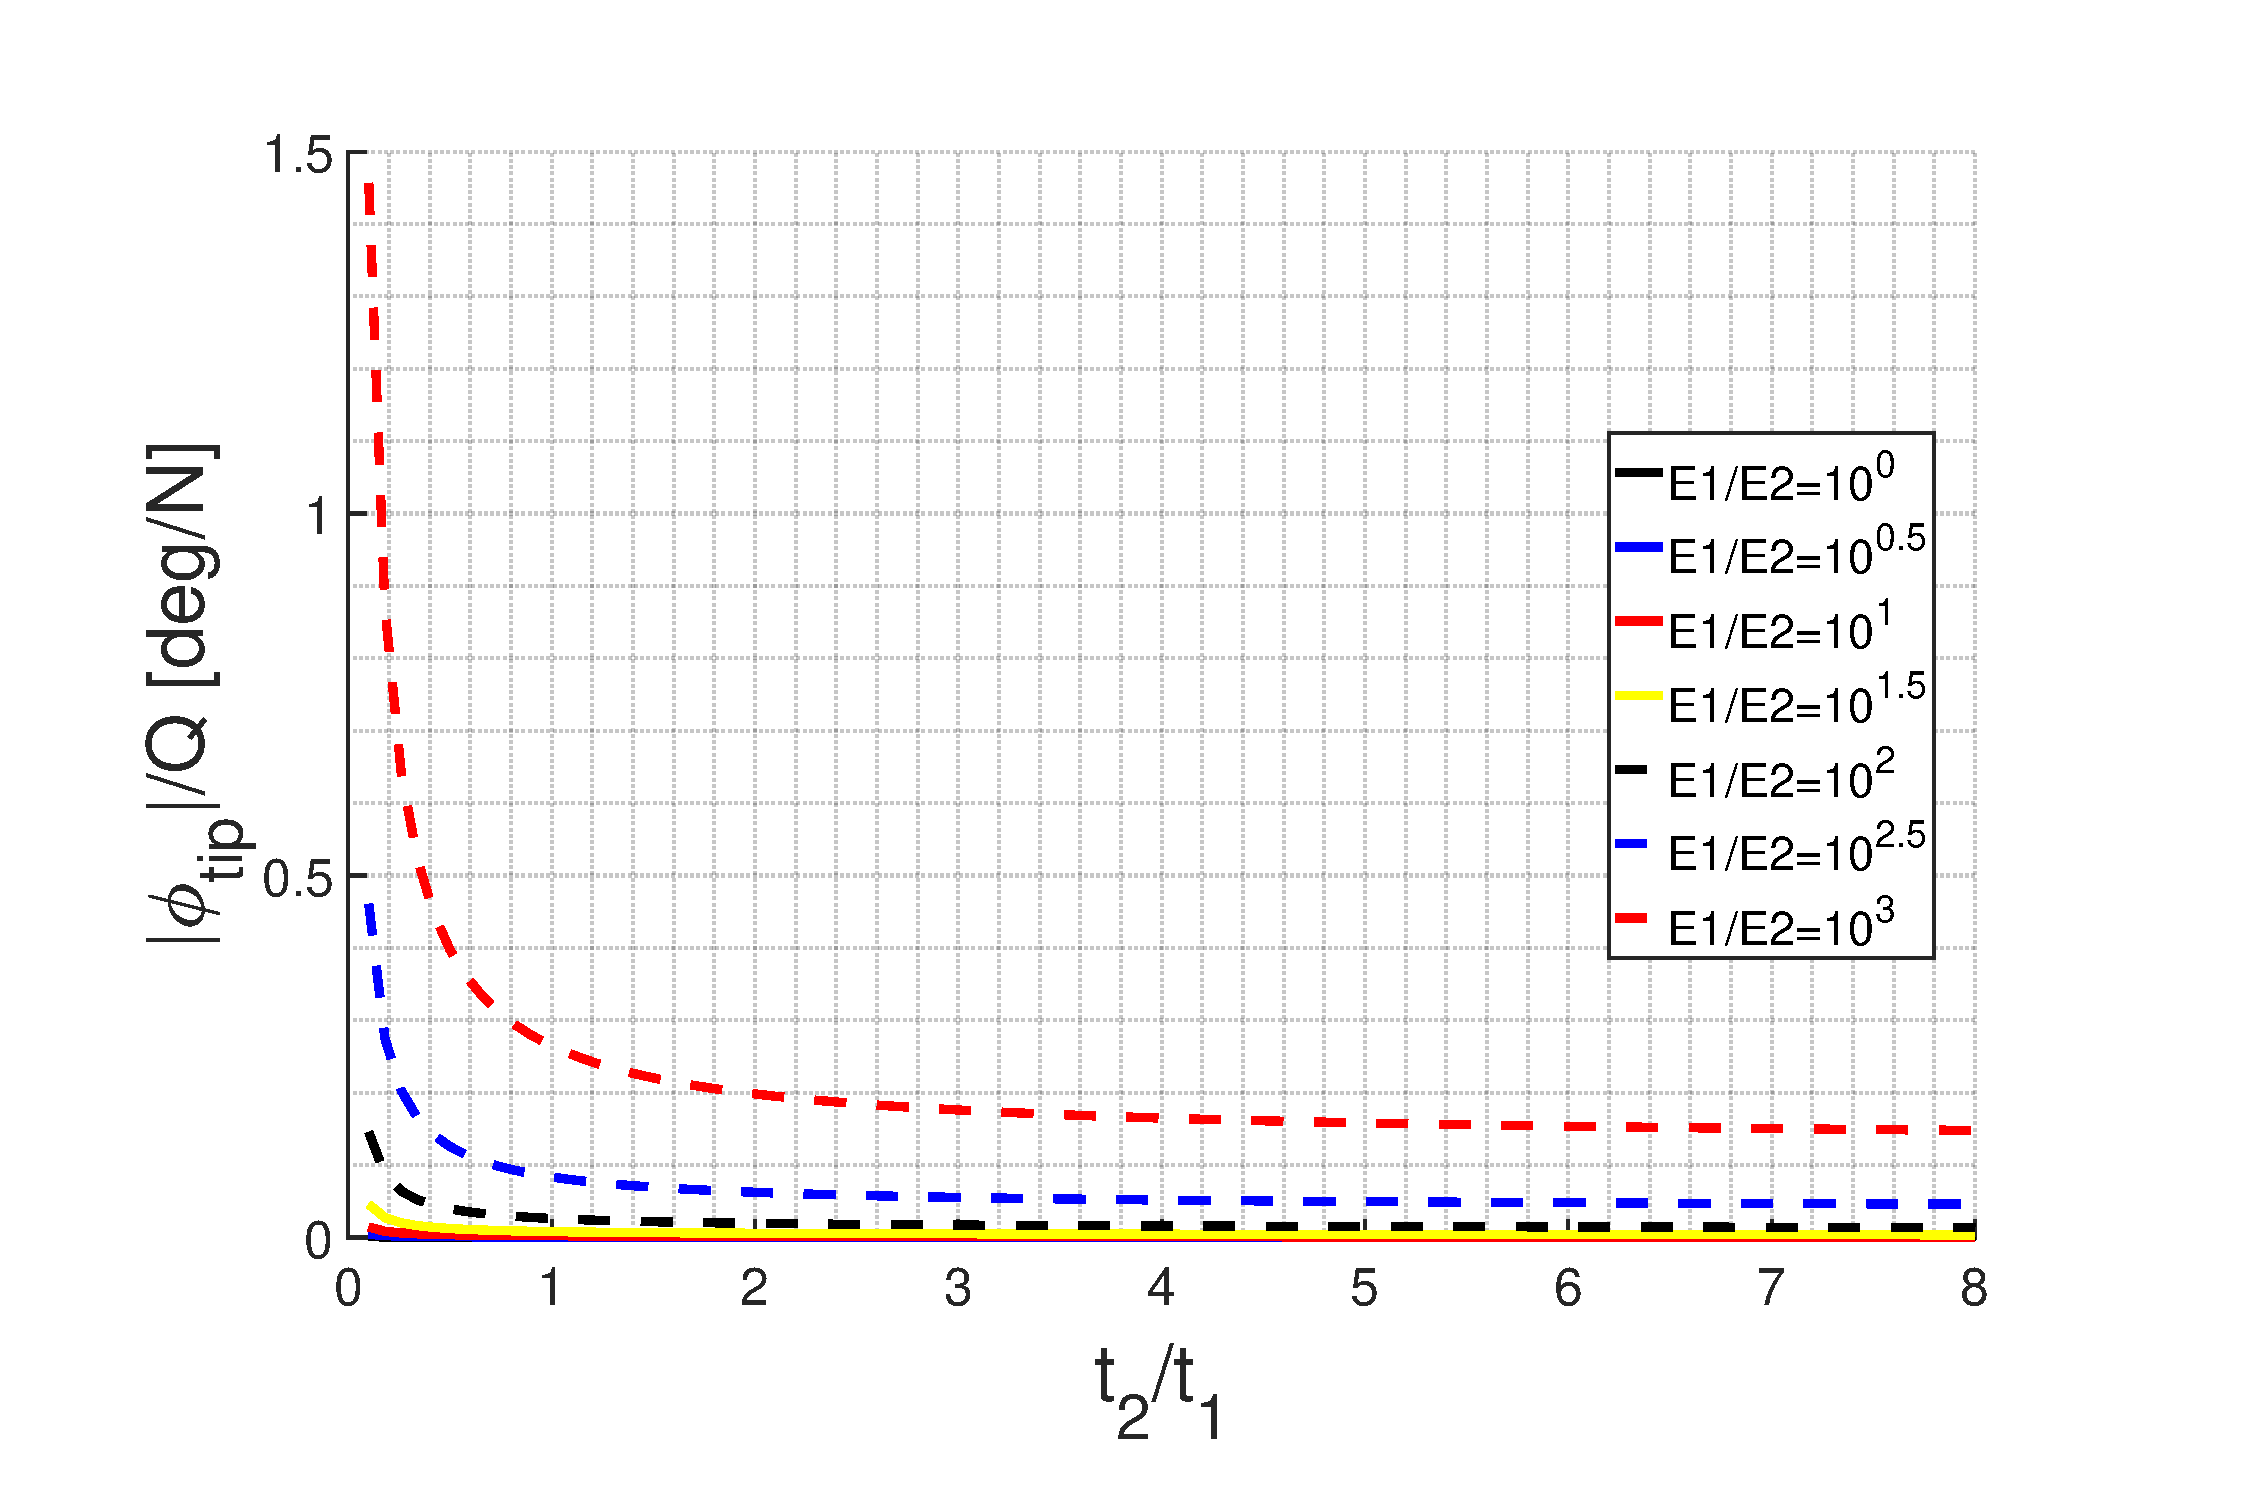
\includegraphics[width=0.8 \textwidth]{../../analytical/figures/phioverQ-E1overE2-t2overt1}
  \caption[Influence of the thickness ratio $t2/t1$ on the torsional compliance]{Influence of the thickness ratio $t2/t1$ on the torsional compliance $|\phi_{\mathrm{tip}}| / Q$ is shown for various values of the stiffness ratio $E_1/E_2$ ranging from $10^0$ to $10^3$. }\label{fig:phioverQ-E1overE2-t2overt1}
\end{figure}

%%%% Figures variation of L / B
\begin{figure}[!htpb] %w_0,tip / Q versus L/B, deflection compliance
  \centering
  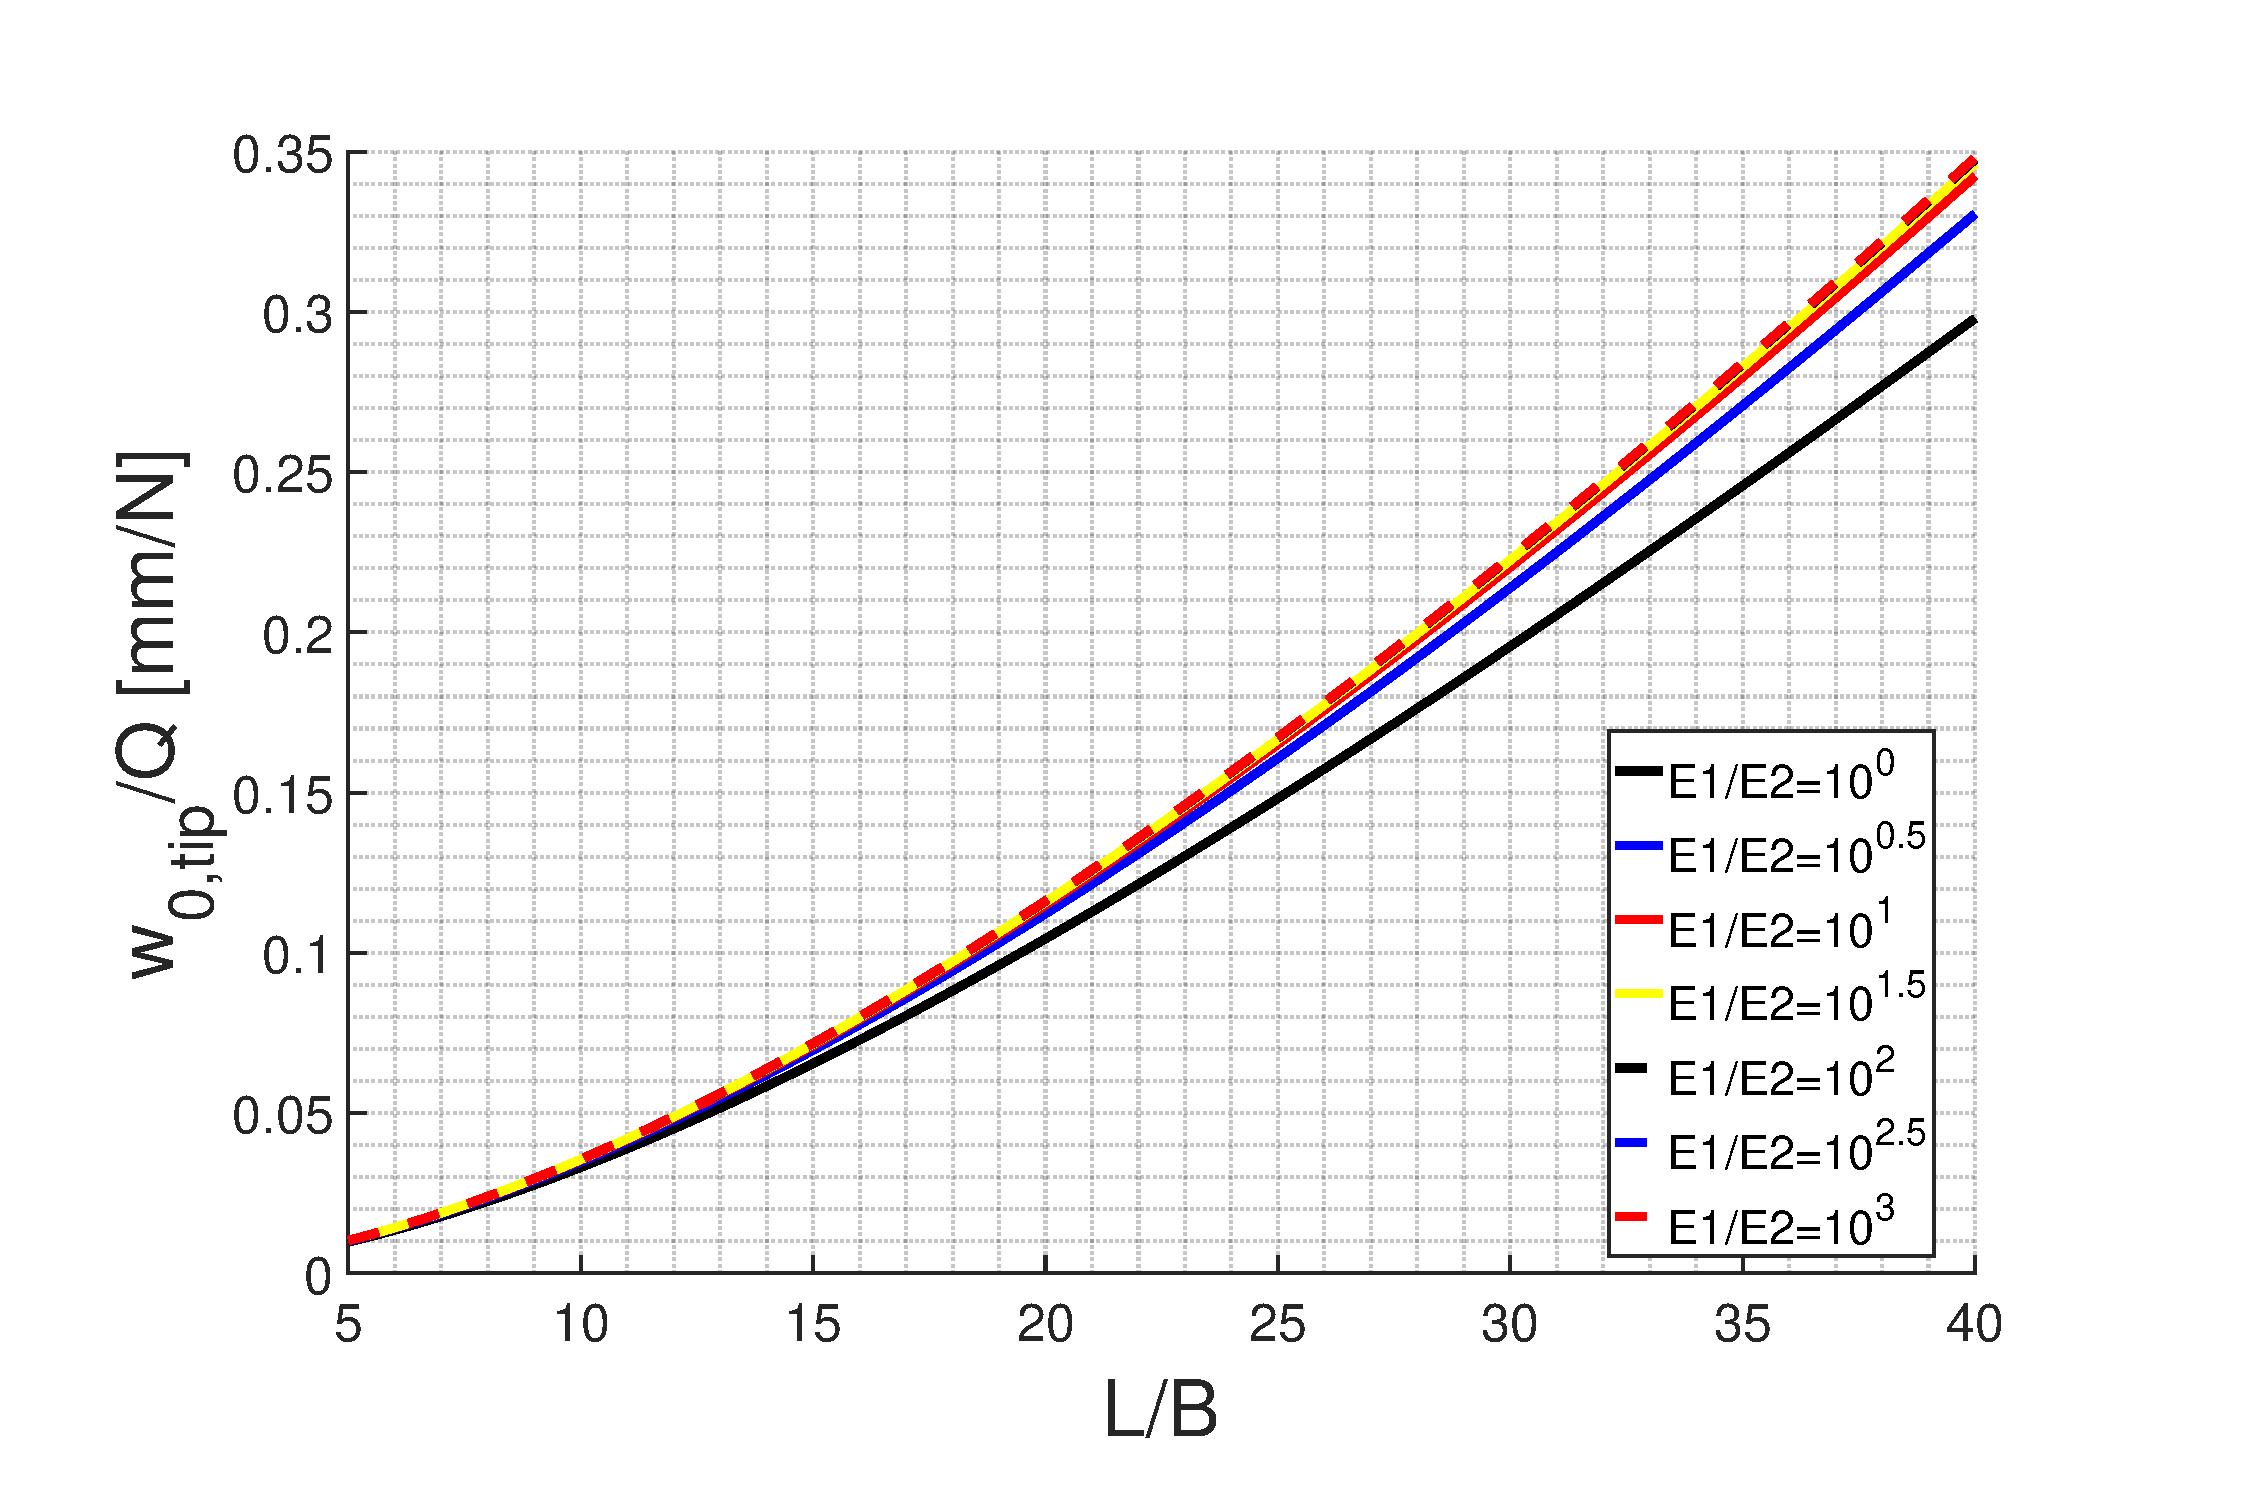
\includegraphics[width=0.8 \textwidth]{../../analytical/figures/woverQ-E1overE2-LoverB}
  \caption[Influence of the slenderness ratio $L/B$ on the deflection compliance]{Influence of the slenderness ratio $L/B$ on the deflection compliance $w_{\mathrm{0,tip}} / Q$ is shown for various values of the stiffness ratio $E_1/E_2$ ranging from $10^0$ to $10^3$. }\label{fig:woverQ-E1overE2-LoverB}
\end{figure}

\begin{figure}[!htpb] %\phi_tip / Q versus L/B, torsional compliance
  \centering
  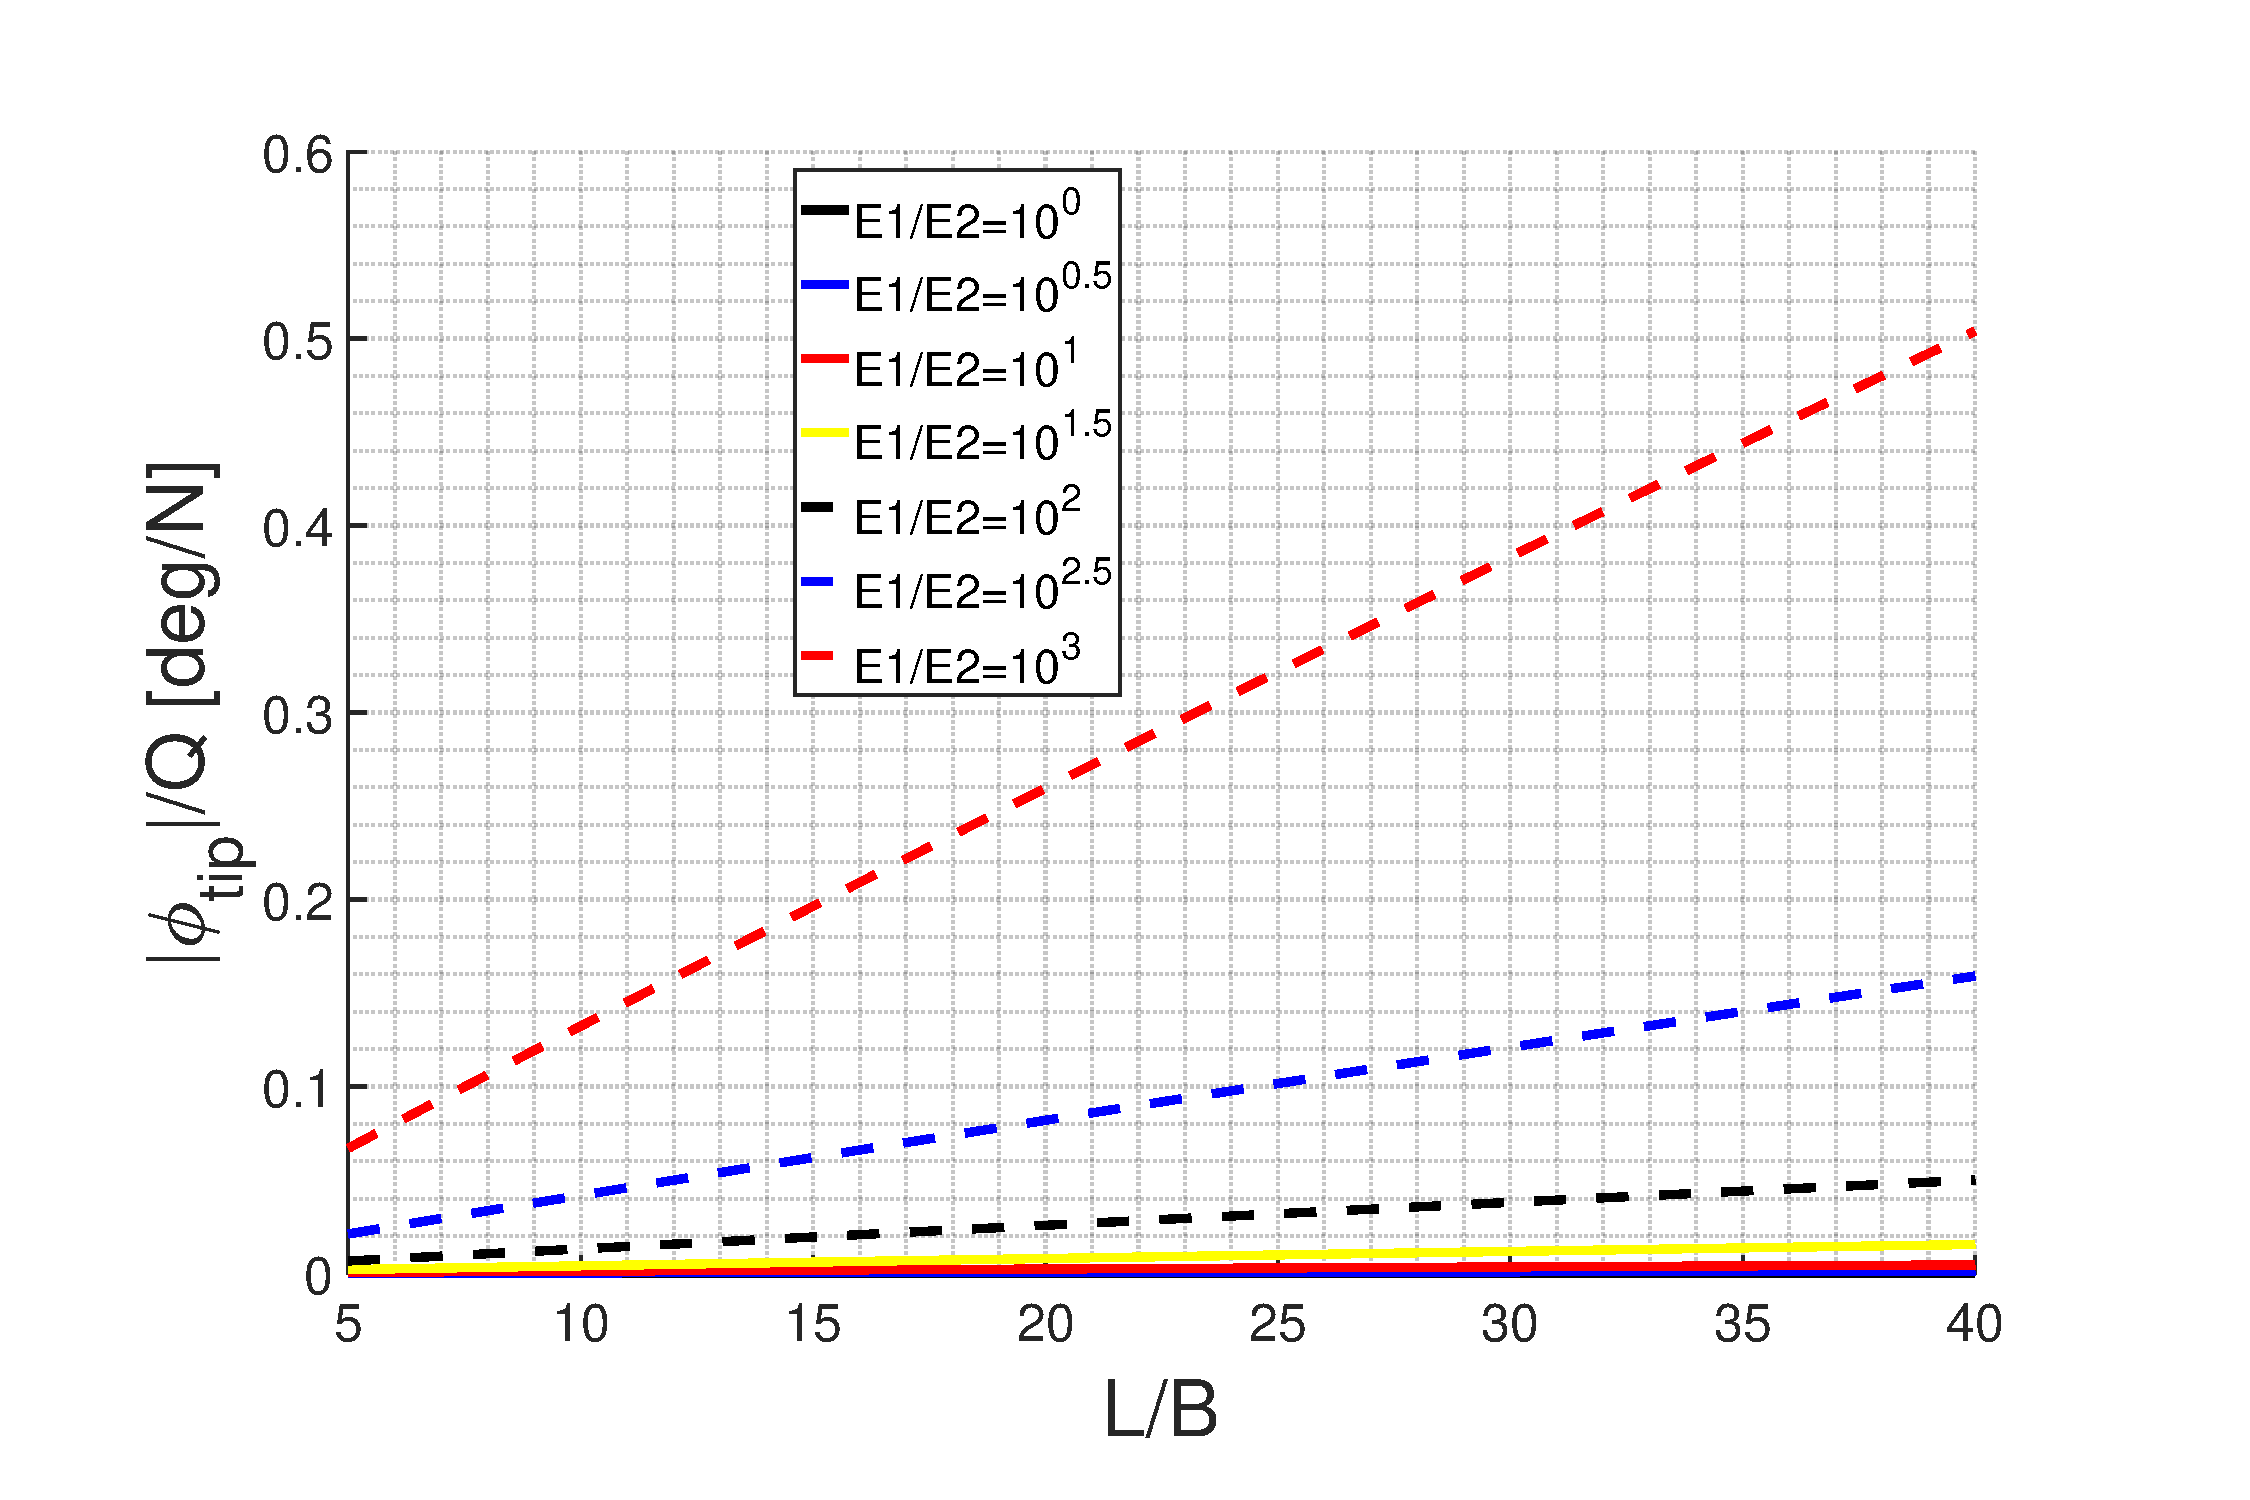
\includegraphics[width=0.8 \textwidth]{../../analytical/figures/phioverQ-E1overE2-LoverB}
  \caption[Influence of the slenderness ratio $L/B$ on the torsional compliance]{Influence of the slenderness ratio $L/B$ on the torsional compliance $|\phi_{\mathrm{tip}}| / Q$ is shown for various values of the stiffness ratio $E_1/E_2$ ranging from $10^0$ to $10^3$. }\label{fig:phioverQ-E1overE2-LoverB}
\end{figure}

\clearpage
\subsubsection{Discussion of the results} \label{subsubsec:disc_results_parametricStudy}

The maximum torsional stiffness $G I_t$ as a function on the cross-sectional aspect ratio $B/H$ can be visualized in Figure \ref{fig:GIt-E1overE2-BoverH}. It can be seen that it appears for $B/H = 1$ when $E_1/E_2 = 1$. Therefore, as it is also shown in \cite{Raither_basic}, the closer the torsional stiffness to the doubly symmetric case, the higher its torsional stiffness. However, when $E_1/E_2 > 10$, the maximum torsional stiffness is shown to appear for $B/H > 1$. A similar conclusion can be extract when analysing the Figure \ref{fig:GIt-E1overE2-t2overt1}, that shows the influence of the thickness ratio $t_2/t_1$ on the torsional stiffness $G I_t$.

In Figure \ref{fig:SC-E1overE2-BoverH} it can be seen that for values $E_2 \ll E_1$, the shear centre position $y_{\mathrm{SC}}$ is approximately constant for $B/H$ variations. In this context, the beam approximates its behavior as if it has an open profile section. However, as the value of $E_1/E_2$ decreases, the influence of the ratio $B/H$ increases showing a bigger influence of the web where the Young's modulus $E_2$ applies. On the other hand, Figure \ref{fig:SC-E1overE2-t2overt1} shows that the bigger the thickness ratio $t_2/t_1$ is, the closer that the shear centre $y_{\mathrm{SC}}$ will be to the vertical axis of simmetry. However, for $E_2 \ll E_1$ the influence of the thickness ratio $t_2/t_1$ is reduced.

The influence of the cross-sectional aspect ratio $B/H$ and the tickness ratio $t_2/t_1$ on the flexural stiffness $E I_y$ is shown to be bigger that that of the Young's modulus ratio $E_1/E_2$, as shown on Figures \ref{fig:EIy-E1overE2-BoverH} and \ref{fig:EIy-E1overE2-t2overt1}, respectively.

% The beam torsional compliance is highly dependant on that torsional moment applied on the beam, that depends on the shear centre $y_{\mathrm{SC}} position. Therefore, as shown on Figure \ref{fig:phioverQ-E1overE2-t2overt1}, the beam's torsional compliance is approximately constant for values of thickness ratio $t_2/t_1 > 1$.


%Comparison of the torsional compliance at the tip against stiffness ratio

\section{Computational model} \label{sec:computationalModel}

% Description of the model
%   Include all the parts of the model: C-box shape, inner box, chiral lattice
%   Figure of the model
% Parameters included
% 